%%%%%%%%%%%%%%%%%%%%%%%%%%%%%%%%%%%%%%%%%%%%%%%%%%%%%%%%%%%%%%%%%%%%%%%%%
%%   CHAPTER: STILL LIFES
%%%%%%%%%%%%%%%%%%%%%%%%%%%%%%%%%%%%%%%%%%%%%%%%%%%%%%%%%%%%%%%%%%%%%%%%%

\renewcommand{\chapterfolder}{still_lifes/}
\chapterimage{cover/still_lifes} % Trees chapter heading image
\chapter{Still Lifes}\index{still life}


\vspace*{-0.4in}
\epigraph{Stand still. The trees ahead and the bushes beside you are not lost.}{David R. Wagoner}
\vspace*{0.4in}


\noindent In this chapter, we investigate the simplest possible objects in Life: those which do not move at all, but rather stay exactly the same from one generation to the next. As we have already learned, such objects are called \emph{still lifes}, and we have seen several examples of them, including the block, tub, boat, ship, beehive, and loaf. Some additional small still lifes are the \emph{aircraft carrier}\index{aircraft carrier}, \emph{barge}\index{barge}, \emph{snake}\index{snake}, \emph{long boat}\index{long boat}, \emph{long snake}\index{long snake}, and \emph{eater~1}\index{eater 1} (see Figure~\ref{fig:small_still_lifes}). In fact, we have just listed every single still life with $7$ or fewer live cells.
\begin{figure}[!htb]
	\centering\begin{tikzpicture}[scale=0.9, every node/.style={transform shape}]%
		\node[inner sep=0pt,anchor=south west] at (0,0) {\patternimglink{0.135}{small_still_lifes}};
		
		\colorletternode{gray}{0}{4}{4}
		\colorletternode{gray}{4.1}{4}{6}
		\colorletternode{gray}{0.65}{1.7}{5}
		\colorletternode{gray}{4.55}{1.7}{7}
	\end{tikzpicture}
	\caption{All still lifes with $7$ or fewer live cells, arranged by their cell count. From left to right: ($4$ cells) block, tub, ($5$ cells) boat, ($6$ cells), snake, ship, beehive, aircraft carrier, barge, ($7$ cells) long snake, long boat, loaf, and eater~1 (which is sometimes called \emph{fishhook}\index{fishhook}).}\label{fig:small_still_lifes}
\end{figure}

While it might seem like there is not much to say about such simple objects, they actually have a somewhat complicated structure and some interesting connections to other areas of mathematics. Furthermore, familiarity with still lifes, especially the small common ones, will be extremely important when constructing larger and more complicated patterns---we already saw this in the previous chapter, where we strategically used blocks to turn queen bees and twin bees into oscillators and glider guns.


%%%%%%%%%%%%%%%%%%%%%%%%%%%%%%%%%%%%%%%%%%%%%%%%%%%%%%%%%%%%%%%%%%%%%%%%%
%%   SECTION: STRICT AND PSEUDO STILL LIFES
%%%%%%%%%%%%%%%%%%%%%%%%%%%%%%%%%%%%%%%%%%%%%%%%%%%%%%%%%%%%%%%%%%%%%%%%%
\section{Strict and Pseudo Still Lifes}\label{sec:pseudo_strict_still_lifes}

We saw in Figure~\ref{fig:small_still_lifes} a complete list of all still lifes with $7$ or fewer cells. We would like to continue in this way and create exhaustive lists of all still lifes with $8, 9, 10, \ldots$ live cells as well, but something strange happens in these cases---we have the freedom to place multiple disjoint copies of still lifes at various places in the plane. For example, we could place two blocks far away from each other at various locations, thus creating an infinite collection of (trivial) $8$-cell still lifes.

Still lifes constructed in this way are in a sense not really any different from their component still lifes, so we would like to ignore them when creating exhaustive lists like this. With this in mind, we define a \emph{strict still life} to be a still life that is either connected, or is disconnected but its different connected components cannot be partitioned into two or more sets that are still lifes by themselves (see Figure~\ref{fig:strict_non_strict}). The reason for not solely restricting our attention to connected still lifes is that some still lifes, like the aircraft carrier, are disconnected yet really are non-trivial---if we separate their two pieces, they are no longer stable.

\begin{figure}[!htb]
	\centering\patternimglink{0.1}{strict_non_strict}
	\caption{From left to right, these still lifes are the beehive, aircraft carrier, \emph{block on table}\index{block on table}, \emph{bi-block}\index{bi-block}, and honey farm\index{honey farm}. The beehive is a strict still life because it is connected, the aircraft carrier is a strict still life because its two halves are not still lifes by themselves but together they overpopulate the cells highlighted in \bgbox{redback}{red}, and the block on table is a strict still life for the same reason. However, the bi-block and honey farm are \emph{not} strict still lifes, since they are made up of non-interacting simpler still lifes.}\label{fig:strict_non_strict}
\end{figure}

However, there is a somewhat weaker notion of whether or not a still life is ``trivial'', and it is highlighted in the difference between the bi-block and the honeyfarm from Figure~\ref{fig:strict_non_strict}. In the bi-block, the two blocks are close enough to each other that they are ``almost touching'' and their Moore neighborhoods overlap, whereas the beehives in the honeyfarm are far enough away from each other that they simply do not interact with each other at all. To capture this difference, we define a \emph{pseudo still life}\index{pseudo!still life} to be a disconnected still life with the property that its connected components can be partitioned into two or more sets that are individually still lifes,\footnote{In the early days of Life, it was not uncommon to define pseudo still lifes as requiring that they can be partitioned into \emph{exactly} two individual still lifes. Matthew Cook demonstrated that the difference between these two definitions is actually quite important, since determining whether or not a pattern can be split into exactly two individual still lifes is relatively easy, whereas determining whether or not it can be split into two \emph{or more} still lifes is quite hard \cite{Coo03}.} and furthermore at least one dead cell has more than $3$ live neighbors in the overall pattern but has fewer than $3$ live neighbors in the subpatterns\footnote{This final restriction is made to capture the notion of the individual connected components ``almost touching''.} (see Figure~\ref{fig:pseudo_not_pseudo} for some examples).

\begin{figure}[!htb]
	\centering\patternimglink{0.1}{pseudo_not_pseudo}
	\caption{From left to right, these are the block, bi-block, two nameless configurations of two blocks, and the blockade\index{blockade}. The bi-block is a pseudo still life because of the cells highlighted in \bgbox{greenpastel}{green} between the blocks that have more than $3$ neighbors. The middle configuration is not a still life at all since the two cells highlighted in \bgbox{redback}{red} will come to life in the next generation. The fourth and fifth configurations are neither strict nor pseudo still lifes, since there is no dead cell that has more than $3$ live neighbors between any of the pairs of blocks---the cell highlighted in \bgbox{yellowback2}{yellow} is in the neighborhood of both blocks, but is still underpopulated (see Exercise~\ref{exer:quasi_still_life}).}\label{fig:pseudo_not_pseudo}
\end{figure}

\begin{table}[!htp]
	\begin{center}		
		\begin{tabular}{Sc Sc Sl Sc Sl}
			\toprule
			Cells & \# of Strict & Examples & \# of Pseudo & Example \\\midrule
			\specialcell{4} & \specialcell{2} & \embedlink{small_still_lifes_table}{\specialcell{\patternimg{0.1}{sl_table_4_strict}}} & \specialcell{0} & \specialcell{--} \\
			
			\rowcolor{gray!20} \specialcell{5} & \specialcell{1} & \specialcell{\patternlink{small_still_lifes_table}{\patternimg{0.1}{sl_table_5_strict}}} & \specialcell{0} & \specialcell{--} \\
			
			\specialcell{6} & \specialcell{5} & \specialcell{\patternlink{small_still_lifes_table}{\patternimg{0.1}{sl_table_6_strict}}} & \specialcell{0} & \specialcell{--} \\
			
			\rowcolor{gray!20} \specialcell{7} & \specialcell{4} & \specialcell{\patternlink{small_still_lifes_table}{\patternimg{0.1}{sl_table_7_strict}}} & \specialcell{0} & \specialcell{--} \\
			
			\specialcell{8} & \specialcell{9} & \specialcell{\patternlink{small_still_lifes_table}{\patternimg{0.1}{sl_table_8_strict}}} & \specialcell{1} & \specialcell{\patternlink{small_still_lifes_table}{\patternimg{0.1}{sl_table_8_pseudo}}} \\
			
			\rowcolor{gray!20} \specialcell{9} & \specialcell{10} & \specialcell{\patternlink{small_still_lifes_table}{\patternimg{0.1}{sl_table_9_strict}}} & \specialcell{1} & \specialcell{\patternlink{small_still_lifes_table}{\patternimg{0.1}{sl_table_9_pseudo}}} \\
			
			\specialcell{10} & \specialcell{25} & \specialcell{\patternlink{small_still_lifes_table}{\patternimg{0.1}{sl_table_10_strict}}} & \specialcell{7} & \specialcell{\patternlink{small_still_lifes_table}{\patternimg{0.1}{sl_table_10_pseudo}}} \\
			
			\rowcolor{gray!20} \specialcell{11} & \specialcell{46} & \specialcell{\patternlink{small_still_lifes_table}{\patternimg{0.1}{sl_table_11_strict}}} & \specialcell{16} & \specialcell{\patternlink{small_still_lifes_table}{\patternimg{0.1}{sl_table_11_pseudo}}} \\
			
			\specialcell{12} & \specialcell{121} & \specialcell{\patternlink{small_still_lifes_table}{\patternimg{0.1}{sl_table_12_strict}}} & \specialcell{55} & \specialcell{\patternlink{small_still_lifes_table}{\patternimg{0.1}{sl_table_12_pseudo}}} \\
			
			\rowcolor{gray!20} \specialcell{13} & \specialcell{240} & \specialcell{\patternlink{small_still_lifes_table}{\patternimg{0.1}{sl_table_13_strict}}} & \specialcell{110} & \specialcell{\patternlink{small_still_lifes_table}{\patternimg{0.1}{sl_table_13_pseudo}}} \\
			
			\specialcell{14} & \specialcell{619} & \specialcell{\patternlink{small_still_lifes_table}{\patternimg{0.1}{sl_table_14_strict}}} & \specialcell{279} & \specialcell{\patternlink{small_still_lifes_table}{\patternimg{0.1}{sl_table_14_pseudo}}} \\
			
			\rowcolor{gray!20} \specialcell{15} & \specialcell{1,353} & \specialcell{\patternlink{small_still_lifes_table}{\patternimg{0.1}{sl_table_15_strict}}} & \specialcell{620} & \specialcell{\patternlink{small_still_lifes_table}{\patternimg{0.1}{sl_table_15_pseudo}}} \\
			
			\specialcell{16} & \specialcell{3,286} & \specialcell{\patternlink{small_still_lifes_table}{\patternimg{0.1}{sl_table_16_strict}}} & \specialcell{1,645} & \specialcell{\patternlink{small_still_lifes_table}{\patternimg{0.1}{sl_table_16_pseudo}}} \\
			
			\rowcolor{gray!20} \specialcell{17} & \specialcell{7,773} & \specialcell{\patternlink{small_still_lifes_table}{\patternimg{0.1}{sl_table_17_strict}}} & \specialcell{4,067} & \specialcell{\patternlink{small_still_lifes_table}{\patternimg{0.1}{sl_table_17_pseudo}}} \\
			
			\specialcell{18} & \specialcell{19,044} & \specialcell{\patternlink{small_still_lifes_table}{\patternimg{0.1}{sl_table_18_strict}}} & \specialcell{10,843} & \specialcell{\patternlink{small_still_lifes_table}{\patternimg{0.1}{sl_table_18_pseudo}}} \\
			
			\rowcolor{gray!20} \specialcell{19} & \specialcell{45,759} & \specialcell{\patternlink{small_still_lifes_table}{\patternimg{0.1}{sl_table_19_strict}}} & \specialcell{27,250} & \specialcell{\patternlink{small_still_lifes_table}{\patternimg{0.1}{sl_table_19_pseudo}}} \\
			
			\specialcell{20} & \specialcell{112,243} & \specialcell{\patternlink{small_still_lifes_table}{\patternimg{0.1}{sl_table_20_strict}}} & \specialcell{70,637} & \specialcell{\patternlink{small_still_lifes_table}{\patternimg{0.1}{sl_table_20_pseudo}}} \\
			
			\rowcolor{gray!20} \specialcell{21} & \specialcell{273,188} & \specialcell{\patternlink{small_still_lifes_table}{\patternimg{0.1}{sl_table_21_strict}}} & \specialcell{179,011} & \specialcell{\patternlink{small_still_lifes_table}{\patternimg{0.1}{sl_table_21_pseudo}}} \\
			
			\specialcell{22} & \specialcell{672,172} & \specialcell{\patternlink{small_still_lifes_table}{\patternimg{0.1}{sl_table_22_strict}}} & \specialcell{462,086} & \specialcell{\patternlink{small_still_lifes_table}{\patternimg{0.1}{sl_table_22_pseudo}}} \\
			
			\rowcolor{gray!20} \specialcell{23} & \specialcell{1,646,147} & \specialcell{\patternlink{small_still_lifes_table}{\patternimg{0.1}{sl_table_23_strict}}} & \specialcell{1,184,882} & \specialcell{\patternlink{small_still_lifes_table}{\patternimg{0.1}{sl_table_23_pseudo}}} \\\bottomrule
		\end{tabular}
		\caption{A summary of the still lifes with $23$ or fewer live cells.}\label{tab:small_still_lifes}
	\end{center}
\end{table}

With these definitions cleared up, we are now able to list the still lifes with small numbers of live cells. Since the number of still lifes with a given number of live cells grows so quickly, we do not explicitly list all of them,\footnote{For a complete list of all still lifes with $18$ or fewer live cells (and massive lists of larger still lifes as well), see Mark Niemiec's Life pages at \httpsurl{conwaylife.com/ref/mniemiec/lifepage.htm}.} and instead we just say how many there are of each size and give a few examples in Table~\ref{tab:small_still_lifes}. For space reasons, we only list the number of still lifes up to $23$~cells in size, but we note that they have been computed up to $34$~cells \cite{A019473,A056613}.

Given that the definition of a pseudo still lifes involves being able to partition the still life into $2$ \emph{or more} component still lifes, it seems natural to ask whether or not there really are cases that can be decomposed into (for example) $3$ still lifes but not $2$. Still lifes with this property are indeed known, and the smallest such example is displayed in Figure~\ref{fig:triple_pseudo_still_life}. Similarly, there are pseudo still lifes that can be decomposed into $4$ still lifes, but not $2$ or $3$, such as the one shown in Figure~\ref{fig:quad_pseudo_still_life}.\footnote{The first pseudo still lifes with these properties were found by Matthew Cook around 1998. These slightly smaller ones were found by Gabriel Nivasch in 2001, and they were proved to be minimal via computer search in early 2020.} Somewhat surprisingly, this pattern does not continue: there does \emph{not} exist a pseudo still life that can only be partitioned into $5$ or more still lifes.

\begin{figure}[!htb]
	\begin{subfigure}{.48\textwidth}
		\centering
		\patternimglink{0.1}{triple_pseudo_still_life}
		\caption{A pseudo still life that can be partitioned into $3$ still lifes, but not $2$.}
		\label{fig:triple_pseudo_still_life}
	\end{subfigure} \quad % 
	\begin{subfigure}{.48\textwidth}
		\centering
		\patternimglink{0.098}{quad_pseudo_still_life}
		\caption{A pseudo still life that can be partitioned into $4$ still lifes, but not $2$ or $3$.}
		\label{fig:quad_pseudo_still_life}
	\end{subfigure}
	\caption{Pseudo still lifes that can be partitioned into (a) $3$ still lifes  and (b) $4$ still lifes, but not fewer. The way of partitioning the still lifes is indicated by the different colors.}\label{fig:pseudo_still_life_decompose}
\end{figure}

\begin{theorem}\label{thm:pseudo_still_four}
	Every pseudo still life can be partitioned into $4$ or fewer still lifes.
\end{theorem}

\begin{proof}
	First, partition the pseudo still life into its (perhaps much more than $4$) strict still life components. Around each of those strict still lifes, outline the region that extends by 1/2 cell in all directions, as demonstrated in Figure~\ref{fig:messy_pseudo_still_life_map}. The resulting regions do not overlap except for perhaps sharing borders with each other, so the four color theorem\footnote{The four-color theorem is a famous (and notoriously difficult to prove) mathematical result that says that if we separate a 2D plane into regions, we can always use four or fewer colors to color the regions in such a way that no two adjacent regions have the same color.} says that we can use four colors to color these regions in such a way that no two regions with a common border have the same color.\footnote{Regions that only touch at a corner are allowed to have the same color.}
	
	\begin{figure}[!htb]
		\centering
		\begin{tabular}{@{}cccc@{}}
			\begin{subfigure}{.23\textwidth}
				\centering
				\patternimglink{0.085}{messy_pseudo_still_life}
				\caption{A pseudo still life that we want to partition into four stable sub-patterns.}
				\label{fig:messy_pseudo_still_life}
			\end{subfigure} & % 
			\begin{subfigure}{.23\textwidth}
				\centering
				\patternlink{messy_pseudo_still_life}{\patternimg{0.085}{messy_pseudo_still_life_map}}
				\caption{The regions that extend $1/2$ of a square out from each component strict still life.}
				\label{fig:messy_pseudo_still_life_map}
			\end{subfigure} & %
			\begin{subfigure}{.23\textwidth}
				\centering
				\patternlink{messy_pseudo_still_life}{\patternimg{0.085}{messy_pseudo_still_life_map_colored}}
				\caption{We can color these regions using four or fewer colors, by the four color theorem.}
				\label{fig:messy_pseudo_still_life_map_colored}
			\end{subfigure} & % 
			\begin{subfigure}{.22\textwidth}
				\centering
				\patternlink{messy_pseudo_still_life}{\patternimg{0.085}{messy_pseudo_still_life_colored}}
				\caption{We then partition the pseudo still life according to the coloring.}
				\label{fig:messy_pseudo_still_life_colored}
			\end{subfigure}
		\end{tabular}
		\caption{A demonstration of the proof that every pseudo still life can be partitioned into four (or fewer) sets that are individually stable.}\label{fig:pseudo_four_color_theorem}
	\end{figure}
	
	We claim that if we group the strict still lifes according to the color of the region that they are contained in then each of the (no more than $4$) resulting patterns is a still life. To see this, we note that no bordering regions have the same color, so the only way that some of the strict still lifes that are grouped together can have any cells in common in their Moore neighborhoods is if those neighborhoods overlap at a corner (such as the yellow regions and yellow still lifes near the bottom of Figures~\ref{fig:messy_pseudo_still_life_map_colored} and~\ref{fig:messy_pseudo_still_life_colored}, respectively). However, in this case the in-between dead cell only has two live neighbors and thus the (no more than $4$) configurations of still lifes are all stable.
\end{proof}


%%%%%%%%%%%%%%%%%%%%%%%%%%%%%%%%%%%%%%%%%%%%%%%%%%%%%%%%%%%%%%%%%%%%%%%%%
%%   SECTION: STILL LIFE GRAMMAR
%%%%%%%%%%%%%%%%%%%%%%%%%%%%%%%%%%%%%%%%%%%%%%%%%%%%%%%%%%%%%%%%%%%%%%%%%
\section{Still Life Grammar}\label{sec:still_life_grammar}

We saw in Table~\ref{tab:small_still_lifes} that computers have been used to find all still lifes with small numbers of live cells. However, if we want to find a still life with a certain specific shape or combination of properties, there are typically much easier ways to find one than by using an exhaustive computer search. In this section, we will discuss some of the standard methods for constructing, combining, and extending still lifes.

As a simple first example, we note that many still lifes that we have seen come as parts of large families of still lifes that naturally build upon each other. For example, the long boat is obtained from the boat simply by adding an extra two diagonal cells, and the long ship and barge are similarly obtained from the ship and the tub, respectively. We can repeatedly lengthen any of these still lifes in the same way, adding two cells at a time, to construct (rather trivial) still lifes with any number of cells as in Figure~\ref{fig:tub_boat_ship}.

\begin{figure}[!htb]
	\centering\patternimglink{0.1}{tub_boat_ship}
	\caption{From left to right, these still lifes are the tub, barge, \emph{long barge}\index{long barge}, boat, long boat, \emph{long long boat}\index{long long boat}, ship, \emph{long ship}\index{long ship}, and \emph{long long ship}\index{long long ship}. Each of these still lifes can be made as long as we like by continuing the patterns in the obvious way.}\label{fig:tub_boat_ship}
\end{figure}

Some similar families of still lifes come from the snake and long snake, where now we only have to add a single extra diagonal cell every time that we want to lengthen it, as in Figure~\ref{fig:snake_canoe}.\footnote{These elongated versions of still lifes are denoted by using the ``long'' prefix the number of times that it has been lengthened (e.g., a ``long long snake'' is a snake elongated by $2$ cells). Alternatively, ``very''  and ``extra'' imply $1$ and $2$ extra levels of longness: $(n+1)$-th smallest $=$ long${}^n$ = very${}^{n-1}$ long = extra${}^{n-2}$ long. For example, a long${}^3$ snake is a long long long snake is a very very long snake is an extra long snake.}\index{long}\index{very long}\index{extra long}

\begin{figure}[!htb]
	\centering\begin{tikzpicture}[scale=1.0, every node/.style={transform shape}]%
	\tikzset{cross/.style={cross out, draw=black, minimum size=2*(#1-\pgflinewidth), inner sep=0pt, outer sep=0pt},cross/.default={1}}
	
	\node[inner sep=0pt,anchor=south west] at (0,0) {\patternimglink{0.1}{snake_canoe}};
	
	\draw (9.67,0.68) node[cross=13,red] {};
	\end{tikzpicture}
	\caption{From left to right, these objects are the snake, long snake, \emph{long long snake}\index{long long snake}, \emph{long$^3$ snake}\index{long$^3$ snake}, ship, an object that is not a still life due to the \bgbox{greenpastel}{green} cell coming to life, \emph{canoe}\index{canoe}, and \emph{long canoe}\index{long canoe}. Again, each of these still lifes can be made as long as we like by continuing the patterns.}\label{fig:snake_canoe}
\end{figure}

In all of these examples, the still lifes are made up from two very different components: the central portion that can be repeated indefinitely, and the stabilizing end pieces. The $3$-cell pre-block on the ends of each side of the long snakes and long canoes is one commonly-used end piece, and another one is the $4$-cell \emph{tail}\index{tail} depicted in Figure~\ref{fig:hook_tail}. When naming still lifes that use this component, we typically use the ``with tail'' suffix so that the 4th still life in Figure~\ref{fig:hook_tail_examples}, for example, is called the \emph{tub with tail}.\index{tub with tail}\index{boat with tail}\index{cis}\index{trans}\footnote{Some objects, like the boat, can have a tail added to them in two different ways, so names like \emph{boat with tail} become insufficient for distinguishing between them. We thus use the \emph{cis} and \emph{trans} prefixes (borrowed from organic chemistry) to distinguish cases like this where they were two possible tail orientations. For example, the two boats with tails displayed in the 9-cell strict still life row of Table~\ref{tab:small_still_lifes} are called the \emph{cis-boat with tail} and the \emph{trans-boat with tail}.}

\begin{figure}[!htb]
	\centering
	\begin{minipage}[b]{.31\textwidth}
		\centering
		\patternimg{0.1}{hook_tail}
		\caption{A pre-block (left) and a \emph{tail} (right) are two common ways of stabilizing objects (typically when the cells highlighted in \bgbox{aquaback}{aqua} are alive).}
		\label{fig:hook_tail}
	\end{minipage} \quad %
	\begin{minipage}[b]{.64\textwidth}
		\centering
		\patternimglink{0.1}{hook_tail_examples}
		\caption{Several examples of still lifes that use pre-blocks (highlighted in \bgbox{redback}{red}) and tails (highlighted in \bgbox{blueback}{blue}) to stabilize their ends. Note that the tails in the 4th and 5th still lifes are not actually required for stability, but just serve to make the still lifes larger.}
		\label{fig:hook_tail_examples}
	\end{minipage}
\end{figure}

In order to construct larger still lifes, we use the fact that if every cell in a $2 \times 2$ square is alive, then every cell that is an immediate neighbor of that $2 \times 2$ square must be dead (i.e., the $2 \times 2$ square must in fact be a block with a border of dead cells around it) in order for the resulting pattern to be a still life. The reason for this is that each cell in the $2 \times 2$ square already has $3$ live neighbors in that $2 \times 2$ square, so adding another one will overcrowd it, causing it to not be stable.\footnote{The term \emph{stable}\index{stable} is sometimes used to refer to still lifes, and it is sometimes used to refer to both still lifes and oscillators. Which of these two cases is meant is usually clear from context or irrelevant.}

This tells us that still lifes never have ``thick'' sections---they are made up of single-cell-thick ``paths'' of live cells that potentially curve and loop around on themselves, possibly plus some isolated blocks. Furthermore, it is often\footnote{But not always---see Exercise~\ref{exer:still_life_impossible}.} possible to take a single-cell-thick path (which does not have overpopulated cells like in Figure~\ref{fig:invalid_path}) and add extra junk around it to suppress the birth of nearby dead cells, thus resulting in a still life (see Figure~\ref{fig:still_life_path} for an example).

\begin{figure}[!htb]
	\centering
	\begin{minipage}{.31\textwidth}
		\centering
		\patternimg{0.1}{invalid_path}
		\caption{Three path segments that cause overcrowding of the central cell and thus must be avoided in still lifes.}
		\label{fig:invalid_path}
	\end{minipage} \quad %
	\begin{minipage}{.64\textwidth}
		\centering
		\patternimglink{0.1}{still_life_path}
		\caption{A single-cell-thick path of live cells (left) can typically be stabilized by adding other nearby objects and branching paths (right).}
		\label{fig:still_life_path}
	\end{minipage}
\end{figure}

While there is no completely foolproof way of carrying out this procedure (some trial-and-error is typically used), some general rules of thumb include using pre-blocks or tails on the ends of the path, doubling the thickness of diagonal sections of the path, and stabilizing orthogonal sections of the path with either orthogonal sections of a new path or with other still lifes like blocks or snakes. When objects are used to stabilize other (non-touching) nearby objects, like how we used the blocks and the snake in Figure~\ref{fig:still_life_path} to stabilize the top-right section of our original path, they are called \emph{induction coils}.\index{induction coil}

Induction coils are most frequently used along long sections of orthogonally connected live cells. For example, a section of $5$ orthogonally connected live cells can be stabilized by any still life that has a single cell farther in one direction than any of its other cells, such as a tub or an eater~1 (or almost any other still life with a tail), since this single cell overpopulates all $3$ dead cells that would otherwise be born---see Figure~\ref{fig:5_cell_induction}. Blocks and snakes are useful because they can be placed next to each other with gaps of $1$ or $2$ dead cells between them, to stabilize rows of connected cells of any length, as in Figure~\ref{fig:induction_coil_examples} (which also illustrates several other common induction coils).

\begin{figure}[!htb]
	\centering
	\begin{minipage}{.31\textwidth}
		\centering
		\patternimglink{0.1}{5_cell_induction}
		\caption{A tub, a boat, a loaf, a still life with a tail, or any other ``pointy'' still life can be used as an induction coil to prevent the birth of $3$ orthogonally connected cells.}
		\label{fig:5_cell_induction}
	\end{minipage} \quad %
	\begin{minipage}{.64\textwidth}
		\centering
		\patternimglink{0.1}{induction_coil_examples}
		\caption{A demonstration of several induction coils being used to stabilize an object. The induction coil at the top-right corner is the \emph{cap}\index{cap}, in the bottom-middle are a \emph{table}\index{table} and a way of extending it, and at the bottom-right is a \emph{bookend}\index{bookend}.}
		\label{fig:induction_coil_examples}
	\end{minipage}
\end{figure}


%%%%%%%%%%%%%%%%%%%%%%%%%%%%%%%%%%%%%%%%%%%%%%%%%%%%%%%%%%%%%%%%%%%%%%%%%
%%   SECTION: EATERS
%%%%%%%%%%%%%%%%%%%%%%%%%%%%%%%%%%%%%%%%%%%%%%%%%%%%%%%%%%%%%%%%%%%%%%%%%
\section{Eaters}\label{sec:eaters}\index{eater}

Many of the complex patterns that we construct in later sections of this book will be based on sending gliders from one place to another, so we will need simple ways of creating, moving, and deleting gliders. Deleting gliders is the simplest of these tasks, and it can be done with objects called \emph{eaters}: still lifes\footnote{Strictly speaking, an eater does not need to be a still life, but still life eaters are used so much more frequently than other types of eaters that it is often assumed.} with the property that if a glider (or another object) collides with them in the right away, the glider is deleted and the eater suffers no permanent damage.

The smallest, first discovered,\footnote{Eater~1 itself was almost immediately discovered independently by several Life enthusiasts as the smallest asymmetric still life, but its eating properties were discovered by Bill Gosper's group at MIT in 1971.} and most widely-used glider eater is the 7-cell still life called eater~1, whose glider-eating reaction is displayed in Figure~\ref{fig:eater_1}. The reason for eater~1's widespread use is not only due to its small size, but also because it returns to its original state only $4$ generations after being hit by the glider (we thus say that it has a \emph{recovery time}\index{recovery time} of $4$ generations), making it the fastest-recovering known glider eater.\footnote{There are also other glider eaters that tie its recovery time of $4$ generations---see Exercise~\ref{exer:fast_glider_eater}.}

\begin{figure}[!htb]
	\centering
	\embedlink{eater_1_glider}{\vcenteredhbox{\patternimg{0.1}{eater_1_glider_1}} \vcenteredhbox{\genarrow{1}} \vcenteredhbox{\patternimg{0.1}{eater_1_glider_2}} \vcenteredhbox{\genarrow{1}} \vcenteredhbox{\patternimg{0.1}{eater_1_glider_3}} \vcenteredhbox{\genarrow{1}} \vcenteredhbox{\patternimg{0.1}{eater_1_glider_4}} \vcenteredhbox{\genarrow{1}} \vcenteredhbox{\patternimg{0.1}{eater_1_glider_5}}}
	\caption{Eater 1 is a seven-cell still life that takes 4 generations to eat a glider.}\label{fig:eater_1}
\end{figure}

In addition to eating gliders, eater~1 can also be used to eat lightweight spaceships, middleweight spaceships, blinkers, and numerous other objects (see Figure~\ref{fig:eater_1_multi}). The fact that eater~1 remains unaffected by so many different types of debris hitting its top-left corner make it extremely useful not just as an eater, but also as a stabilizer in numerous more complicated patterns. We already demonstrated this phenomenon in Exercise~\ref{exer:queen_bee_eater_1}, where we used eater~1 to stabilize a queen bee, and we will see how eater~1 can be used to construct various other oscillators in Section~\ref{sec:corner_oscillators}. Furthermore, eater~1 will appear repeatedly when we construct glider loops and Herschel tracks in Sections~\ref{sec:glider_loops} and~\ref{sec:herschel_track}, respectively.

\begin{figure}[!htb]
	\centering\embedlink{eater_1_multi}{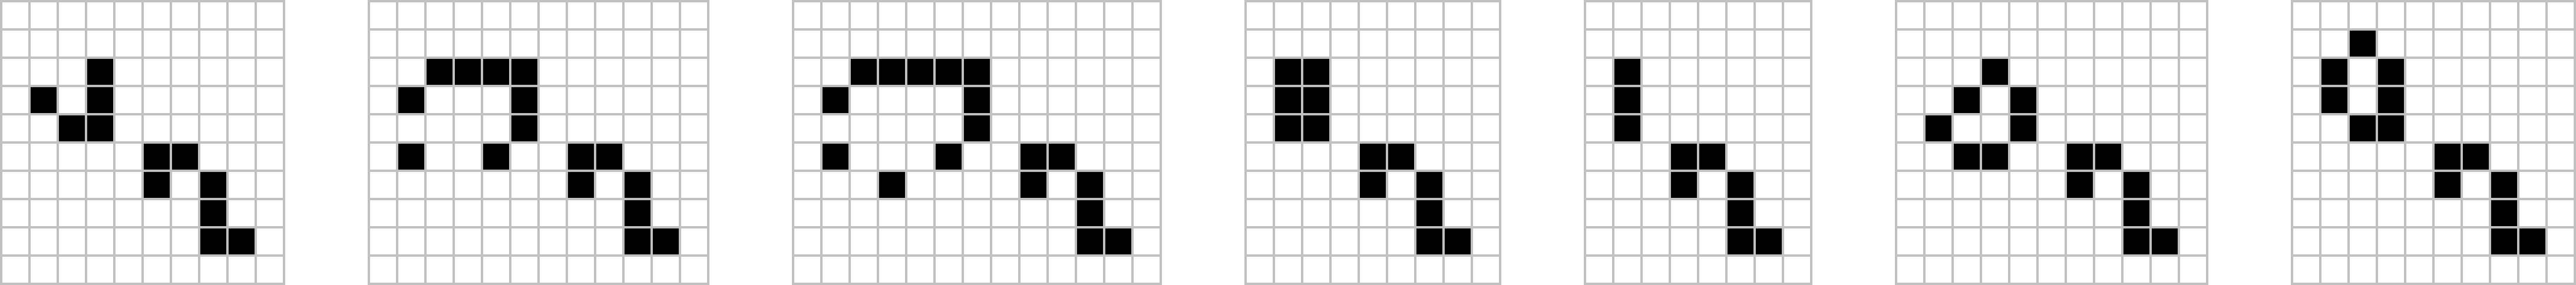
\includegraphics[width=0.9\textwidth]{still_lifes/eater_1_multi.png}}
	\caption{Eater 1 can be used to eat a glider, a lightweight spaceship, a middleweight spaceship, a pre-beehive, and many other objects.}\label{fig:eater_1_multi}
\end{figure}

In spite of the versatility of eater~1, there are other eaters that are sometimes more useful in certain situations. One example is \emph{eater~2} (see Figure~\ref{fig:eater_2}): although it is quite a bit larger than eater~1 and has a recovery time of 5 generations (instead of 4), it has the advantages of being symmetric and being able to eat gliders traveling along 4 different parallel paths.

Similarly, \emph{eater~5} (sometimes called the \emph{tub with tail eater}\index{tub with tail eater}, or \emph{TWIT}\index{TWIT|see {tub with tail eater}} for short) is a small eater\footnote{There are indeed eaters called ``eater~3'' and ``eater~4'' (as well as dozens of other known eaters), but they are somewhat less useful than eaters~1, 2, and~5, so we just introduce these others as we need them.} with a recovery time of 6 generations that is made up of two still lifes and is capable of eating gliders traveling along 2 different perpendicular paths. Eater~5 is is especially useful for the fact that it can eat gliders traveling so close to its edge (in particular, the glider coming from the top-right corner in Figure~\ref{fig:eater_5}), so it can often be used to eat gliders in tight places where other eaters will not fit.

\begin{figure}[!htb]
	\begin{subfigure}{.5\textwidth}
		\centering
		\patternimglink{0.083}{eater_2}
		\caption{Eater~2.}
		\label{fig:eater_2}
	\end{subfigure}% 
	\begin{subfigure}{.5\textwidth}
		\centering
		\patternimglink{0.115}{eater_5}
		\caption{Eater~5.}
		\label{fig:eater_5}
	\end{subfigure}
	\caption{Eater~2 (left) is capable of eating gliders traveling along 4 different parallel paths, while eater~5 (right) is capable of eating gliders traveling along 2 different perpendicular paths.}\label{fig:eater_2_5}
\end{figure}


%%%%%%%%%%%%%%%%%%%%%%%%%%%%%%%%%%%%%%%%%%%%%%%%%%%%%%%%%%%%%%%%%%%%%%%%%
%%   SUBSECTION: ROCKS AND ALMOST EATERS
%%%%%%%%%%%%%%%%%%%%%%%%%%%%%%%%%%%%%%%%%%%%%%%%%%%%%%%%%%%%%%%%%%%%%%%%%
\subsection{Rocks and ``Almost'' Eaters}\label{sec:rocks_almost_eaters}

All of the eaters that we have seen so far are temporarily disturbed when the glider hits them, and then return to their initial state after a few generations. However, there is no fundamental reason that an eater has to be disturbed by the object that it eats at all---an eater is called a \emph{rock} if it does not even suffer temporary damage during the eating process. While there are no known rocks that eat gliders, there are rocks that eat other objects, and there are objects that can act as rocks for \emph{multiple} gliders.

Here we present an example of the latter kind---an object that can destroy two gliders, suffer no damage in the process, yet cannot completely destroy just a single glider. In fact, this object is simply the snake\index{snake}, which is capable of turning a single glider into a boat\index{boat}, which then destroys (and is destroyed by) a second glider coming in from the same direction as the first. This reaction is called the \emph{boat-bit},\index{boat-bit}\footnote{Its name comes from the fact that this reaction can be used to store a single bit of memory. We will explore methods like this one for simulating computation in Chapter~\ref{chp:universal_computation}.} and is displayed in Figure~\ref{fig:boat_bit}.

\begin{figure}[!htb]
	\centering
	\embedlink{boat_bit}{\vcenteredhbox{\patternimg{0.1}{boat_bit_0}} \vcenteredhbox{\genarrow{4}} \vcenteredhbox{\patternimg{0.1}{boat_bit_4}} \vcenteredhbox{\genarrow{20}} \vcenteredhbox{\patternimg{0.1}{boat_bit_24}}}
	\caption{A \emph{boat-bit} is a reaction in which a snake (or any other still life containing a pre-block) is used to turn a glider into a boat which then destroys a second glider coming in from the same position. Furthermore, the snake is not even temporarily disturbed at any point throughout this reaction.}\label{fig:boat_bit}
\end{figure}

While the snake is not technically an eater since it does not destroy each glider that hits it, but rather only destroys pairs of gliders, this is a technicality that is often unimportant. Typically when eating gliders, an entire stream of gliders (perhaps from a glider gun) are fired from the same position, and this boat-bit reaction gives the smallest known way of erasing such a glider stream (in particular, it contains only $6$ cells and is slightly more compact than the $7$-cell eater~1).

There are also many other reactions that use gliders to toggle a Life object between two or more different states, and they can almost all be used to eat multiple glider streams (though they are often useful for much more than this). For example, a single glider can be used to flip the orientation of a loaf\index{loaf}, so a loaf can use this reaction twice to eat two gliders and end up back where it started, as in Figure~\ref{fig:glider_loaf_flip}. Again, a loaf by itself is not technically an eater since it cannot reconstruct itself after destroying a \emph{single} glider, but we can turn it into an eater by placing a stable object next to it that will flip it back over after a glider hits it. One way of doing this results in the eater called \emph{eater~3}\index{eater 3}, which is displayed in Figure~\ref{fig:eater_3}.

\begin{figure}[!htb]
	\centering
	\begin{minipage}{.61\textwidth}
		\centering
		\embedlink{glider_loaf_flip}{\vcenteredhbox{\patternimg{0.1}{glider_loaf_flip}} \vcenteredhbox{\genarrow{4}} \vcenteredhbox{\patternimg{0.1}{glider_loaf_flip_4}} \vcenteredhbox{\genarrow{4}} \vcenteredhbox{\patternimg{0.1}{glider_loaf_flip_8}}}
		\caption{A glider can be used to flip a loaf. A loaf can thus be used to eat two gliders coming from opposite directions.}\label{fig:glider_loaf_flip}
	\end{minipage} \quad %
	\begin{minipage}{.33\textwidth}
		\centering
		\patternimglink{0.092899408284}{eater_3}
		\caption{\emph{Eater 3} is based on the loaf-flipping reaction.}
		\label{fig:eater_3}
	\end{minipage}
\end{figure}

Finally, recall from Section~\ref{sec:queen_bee} that a block\index{block} is the smallest eater of all, as it can be used to eat a beehive (and for that matter, it can also eat a loaf). It can't be used to eat a single glider or even a single glider stream, but it can be used (like a loaf) to eat two gliders coming from opposite directions. This is possible because of the \emph{(2,1) block pull} reaction\index{(2,1) block pull} displayed in Figure~\ref{fig:glider_block_move}, in which a glider is destroyed while moving a block by $2$ cells horizontally and $1$ cell vertically. A second glider coming from the opposite direction then moves the block back to where it started.

While this reaction is perhaps of limited use when it comes to eating gliders (since the opposing gliders have to be positioned exactly right in order to return the block to its starting point), the general idea of using gliders to move blocks around the Life plane is a very useful one that we will explore in depth in Sections~\ref{sec:slow_salvo} and~\ref{sec:slide_guns}.\footnote{We will also see another use of colliding gliders with a block in Exercise~\ref{exer:rephaser}.}

\begin{figure}[!htb]
	\centering
	\embedlink{glider_block_move}{\vcenteredhbox{\patternimg{0.1}{glider_block_move}} \vcenteredhbox{\genarrow{14}} \vcenteredhbox{\patternimg{0.1}{glider_block_move_14}} \vcenteredhbox{\genarrow{8}} \vcenteredhbox{\patternimg{0.1}{glider_block_move_22}}}
	\caption{A \emph{(2,1) block pull} is a reaction in which a glider pulls a block by $2$ cells in one direction and $1$ cell in the other. A block can thus be used to eat two gliders coming from opposite directions.}\label{fig:glider_block_move}
\end{figure}


%%%%%%%%%%%%%%%%%%%%%%%%%%%%%%%%%%%%%%%%%%%%%%%%%%%%%%%%%%%%%%%%%%%%%%%%%
%%   SECTION: WELDING STILL LIFES
%%%%%%%%%%%%%%%%%%%%%%%%%%%%%%%%%%%%%%%%%%%%%%%%%%%%%%%%%%%%%%%%%%%%%%%%%
\section{Welded and Constrained Still Lifes}\label{sec:welding}

We saw in Section~\ref{sec:still_life_grammar} that there are many general methods for constructing a wide variety of still lifes of almost any size. We now focus on using these methods to combine multiple still lifes into a single still life that retains the properties of each of its components (such as the ability to eat gliders that are on specific paths)---a process that is called \emph{welding}.\index{welding}

To give an example of why we might want to weld two still lifes, suppose that we want to erase two gliders that are in the position shown in Figure~\ref{fig:unstable_eater_1s_a}. Since those gliders are so close to each other, there is no way to eat each of them with individual eaters such as easter~1---they will interfere with each other and no longer be stable, as shown in Figure~\ref{fig:unstable_eater_1s_b}.

\begin{figure}[!htb]
	\centering
	\begin{subfigure}{.47\textwidth}
		\centering
		\patternimglink{0.1}{unstable_eater_1s}
		\caption{Two gliders that we would like to eat.}
		\label{fig:unstable_eater_1s_a}
	\end{subfigure} \quad % 
	\begin{subfigure}{.47\textwidth}
		\centering
		\patternlink{unstable_eater_1s}{\patternimg{0.1}{unstable_eater_1s_b}}
		\caption{Placing two individual eaters does not work.}
		\label{fig:unstable_eater_1s_b}
	\end{subfigure}
	\caption{The two gliders in~(a) cannot be eaten by individual eater~1s, since they are too close together and the eater~1s will no longer be stable, as in (b). In particular, the dead cells highlighted in \bgbox{greenback}{green} now have $3$ live neighbors and will be born, while the live cells highlighted in \bgbox{redback}{red} now have $4$ live neighbors and will die. Similar problems occur if we try to use other eaters like eater~2 or eater~5 as well.}\label{fig:unstable_eater_1s}
\end{figure}

To get around this problem, we combine two eater~1s into a single, larger eater. The key idea is that the only part of eater~1 that is actually involved in the glider eating reaction from Figure~\ref{fig:eater_1} is its pre-block (i.e., the $3$-cell corner at its top-left)---its tail is just there to stabilize the pre-block. So to weld two eater~1s together, we place their pre-blocks in the appropriate spots and then replace their tails by a single connecting object in such a way that they are \emph{both} stable, as in Figure~\ref{fig:welded_eater_1s_both}. This stabilizing piece is typically constructed using a combination of the grammar that we introduced in Section~\ref{sec:still_life_grammar} and trial-and-error.

\begin{figure}[!ht]
	\centering
	\begin{subfigure}{.4\textwidth}
		\centering
		\patternimg{0.1}{welded_eater_1s_inc}
		\caption{A placement of pre-blocks (and a bit of the tails) that eats the two gliders.}
		\label{fig:welded_eater_1s_inc}
	\end{subfigure} \quad \ % 
	\begin{subfigure}{.54\textwidth}
		\centering
		\embedlink{welded_eater_1s}{\vcenteredhbox{\patternimg{0.1}{welded_eater_1s}} \vcenteredhbox{\genarrow{4}}
			\vcenteredhbox{\patternimg{0.1}{welded_eater_1s_done}}}
		\caption{A way of welding two eater~1s together to eat both of the gliders.}
		\label{fig:welded_eater_1s}
	\end{subfigure}
	\caption{In order to weld two eater~1s together to make a single still life capable of eating both gliders, we keep both of their pre-blocks but delete their tails, as in (a). We are then free to choose the \bgbox{gridgray!40}{light gray} cells to be alive or dead, and we want to do so in a way that makes the resulting object a still life. One possibility is shown in~(b).}\label{fig:welded_eater_1s_both}
\end{figure}

Welding these two eater~1s together might seem somewhat silly in isolation---we could just place two eater~1s so as to eat the gliders before they get so close together in the first place---but there are two main reasons why welding can be preferable to just placing individual still lifes far apart:\medskip

\begin{enumerate}
	\item[1)] Later on in this book, we will be constructing large patterns that are made up of many other smaller patterns. Some of these sub-patterns might get in our way and restrict the amount of space we have to place the individual still lifes.\smallskip
	
	\item[2)] Similarly, because these large patterns that we will construct are already very large, it is often desirable to reduce their size as much as possible, by packing their components as close together as we can without them colliding. Welding still lifes is one of the main techniques for achieving tight packings of components.\medskip
\end{enumerate}

To give an example that highlights point~(1) above, consider the problem of eating a glider that is positioned as in Figure~\ref{fig:eater_constrained_pre}, but under the restriction that the eater must be contained within the indicated region of the Life plane. Neither eater~1 nor eater~2 come even close to working---if they are positioned in such a way as to eat the glider, they both extend several rows outside of the specified region. However, eater~5 \emph{almost} works---it extends $2$~cells too far in one direction and just $1$~cell too far in the other (see Figure~\ref{fig:eater_constrained_eater_5}).

\begin{figure}[!htb]
	\centering
	\begin{subfigure}{.47\textwidth}
		\centering
		\patternimg{0.1}{eater_constrained_pre}
		\caption{We would like to eat this glider, but our eater must be contained in the \bgbox{gridgray!40}{light gray} region.}
		\label{fig:eater_constrained_pre}
	\end{subfigure} \quad \ % 
	\begin{subfigure}{.47\textwidth}
		\centering
		\patternimg{0.1}{eater_constrained_eater_5}
		\caption{An eater~5 almost works, but sticks just a bit outside of the light gray region.}
		\label{fig:eater_constrained_eater_5}
	\end{subfigure}
	\caption{We are presented with the problem of eating the glider displayed in (a), but under the restriction that the eater we use must live entirely within the light gray region. The only eater that we have seen so far that even comes close to satisfying this restriction is eater~5, so we use that as our starting point in (b).}\label{fig:eater_constrained_eater_5_first}
\end{figure}

To make this eater fit within the specified region, we keep all of the live cells within the region, discard those outside of the region, and then try to add more live cells within the region in order to restore stability and its eating ability. We quickly find that we need to add some live cells to the left and to the bottom-left of the tub in order for the eating reaction to still work.

However, placing live cells near a tub is difficult to do while preserving stability, so we change the tub to a boat and arrive at the pattern in Figure~\ref{fig:eater_constrained_eater_5_b}. This pattern would work as an eater if it were stable, but unfortunately two nearby dead cells come to life in the next generation. To fix this problem, we just extend the pattern to the west and south so as to overpopulate those two cells, until we eventually arrive at a pattern that is completely stable, as in Figure~\ref{fig:eater_constrained_done}. This eater is extremely useful precisely because it eats a glider so close to its corner, and we will make heavy use of it in Section~\ref{sec:herschel_track}.

\begin{figure}[!htb]
	\centering
	\begin{subfigure}{.4\textwidth}
		\centering
		\patternimglink{0.1}{eater_constrained_eater_5_b}
		\caption{An eater that almost works, but is not stable due to the two dead \bgbox{greenback}{green} cells that come to life in the next generation.}
		\label{fig:eater_constrained_eater_5_b}
	\end{subfigure} \quad \ % 
	\begin{subfigure}{.54\textwidth}
		\centering
		\embedlink{eater_constrained_done}{\vcenteredhbox{\patternimg{0.1}{eater_constrained_done}} \vcenteredhbox{\genarrow{6}}
			\vcenteredhbox{\patternimg{0.1}{eater_constrained_done_6}}}
		\caption{We can add additional live cells to the west and south in order to overpopulate the two problematic cells, resulting in an eater that works.}
		\label{fig:eater_constrained_done}
	\end{subfigure}
	\caption{An illustration of one way of transforming eater~5 into an eater that fits within the \bgbox{gridgray!40}{light gray} region. The pattern (a) is not quite stable, since two nearby dead cells come to life in the next generation. The eater depicted in (b) is one solution to this problem, and it has a recovery time of $6$ generations (just like eater~5 itself).}\label{fig:eater_constrained_eater_5_both_done}
\end{figure}


%%%%%%%%%%%%%%%%%%%%%%%%%%%%%%%%%%%%%%%%%%%%%%%%%%%%%%%%%%%%%%%%%%%%%%%%%
%%   SECTION: STILL LIFE DENSITY
%%%%%%%%%%%%%%%%%%%%%%%%%%%%%%%%%%%%%%%%%%%%%%%%%%%%%%%%%%%%%%%%%%%%%%%%%
\section{Still Life Density}\label{sec:still_life_density}

From the very early days of Life, many examples of infinite still lifes were known with density $1/2$. That is, there are many ways of filling the plane in a stable way such that half of the cells are alive and half of them are dead---some examples are presented in Figure~\ref{fig:dense_still_lifes}.
\begin{figure}[!ht]
	\begin{subfigure}{.32\textwidth}
		\centering
		\patternimglink{0.1}{zebra_stripes}
		\caption{\emph{Zebra stripes}.\index{zebra stripes}}
		\label{fig:zebra_stripes}
	\end{subfigure} \ \ %
	\begin{subfigure}{.32\textwidth}
		\centering
		\patternimglink{0.1}{chicken_wire}
		\caption{\emph{Chicken wire}.\index{chicken wire}}
		\label{fig:chicken_wire}
	\end{subfigure} \ \ % 
	\begin{subfigure}{.32\textwidth}
		\centering
		\patternimglink{0.1}{onion_rings}
		\caption{\emph{Onion rings}.\index{onion rings}}
		\label{fig:onion_rings}
	\end{subfigure}
	\caption{When the plane is tiled with these patterns, they create infinite still lifes with density $1/2$.}\label{fig:dense_still_lifes}
\end{figure}

It was a long-standing question whether or not an asymptotic density of greater than $1/2$ is attainable, or if $1/2$ really is the upper limit.\footnote{The conjecture that the asymptotic density of still lifes does not exceed $1/2$ was called the \emph{still life conjecture}, which was first considered in \emph{Lifeline} vol. 3 in September 1971. In 1992, an upper bound of $6/11$ on the density of an infinite still life was proved by Dean Hickerson using the method outlined in Exercise~\ref{exer:sl_density_611}. This bound was then improved to $15/28$ by Hartmut Holzwart, and finally to $1/2$, hence proving the conjecture, by Noam Elkies in 1998 \cite{Elk98}.} The following theorem shows that the latter is the case: there are no stable configurations that are more dense than those presented in Figure~\ref{fig:dense_still_lifes} (though there are others that also attain density~$1/2$).\footnote{The original proof presented in \cite{Elk98} is somewhat complicated and requires a decent amount of casework, but also finds the maximum asymptotic density of still lifes in many other Life-like cellular automata. The simpler proof provided here, which is specific to the Game of Life, was first presented in \cite{CSB09}.}

\begin{theorem}\label{thm:still_life_density}
	A still life contained in an $n \times n$ bounding box has no more than $\lfloor n^2/2 \rfloor + 2n$ live cells. In particular, the asymptotic density of still lifes as $n \rightarrow \infty$ is no greater than $1/2$.
\end{theorem}

\begin{proof}
	We prove the theorem by supposing that each cell (either alive or dead) in the Life plane has $2$ tokens, and we will present a procedure for redistributing those tokens among each cell's orthogonal neighbors (i.e., each token stays within its original von Neumann neighborhood) in such a way that every live cell ends up having at least 4 tokens. If we can develop such a procedure, we know that in any $n \times n$ square there will be at most
	$$
	{\color{gray}\underbrace{\color{black}2n^2}_{\substack{\text{original tokens in} \\ \text{$n \times n$ square}}}} \ + \ {\color{gray}\underbrace{\color{black}8n}_{\substack{\text{tokens from $4n$} \\ \text{neighbors of square}}}} = 2(n^2 + 4n) \text{ tokens.}
	$$
	On the other hand, if there are $L$ live cells in an $n \times n$ square, then since every live cell has at least $4$ tokens we know that
	\begin{align*}
	4L & \leq \text{number of tokens on live cells in $n \times n$ square} \\
	& \leq \text{number of tokens on \emph{all} cells in $n \times n$ square} \\
	& \leq 2(n^2 + 4n).
	\end{align*}
	Dividing this inequality by $4$ gives $L \leq n^2/2 + 2n$, which shows that the asymptotic density of a still life cannot exceed $1/2$.
	
	We thus now turn our attention to developing the token redistribution procedure that results in every live square having at least $4$ tokens (thus proving the theorem). The main idea is to have dead cells give away their tokens to neighboring (in the von Neumann neighborhood sense) live cells. The explicit procedure that we use is described in Figure~\ref{fig:density_orthogonal_neighbors}.
	
	\begin{figure}[!htb]
		\centering\begin{tikzpicture}[scale=1.6, every node/.style={transform shape}]%
		\tikzset{
			double arrow/.style args={#1 colored by #2 and #3}{
				round cap-latex,line width=#1,#2, % first arrow
				postaction={draw,round cap-latex,#3,line width=(#1)/3,
					shorten <=(#1)/3,shorten >=2*(#1)/3}, % second arrow
			}
		}
		
		\node[inner sep=0pt,anchor=south west] at (0,0) {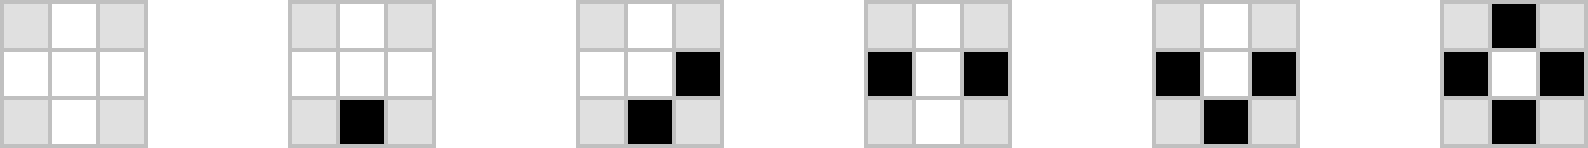
\includegraphics[width=3.3in]{still_lifes/density_orthogonal_neighbors.png}};
		
		\draw[double arrow=4pt colored by white and medgray] (0.755in,0.17in) -- (0.755in,0.04in);
		
		\draw[round cap-latex,line width=4pt,white] (1.355in,0.17in) -- (1.355in,0.04in);
		\draw[round cap-latex,line width=4pt,white] (1.34in,0.155in) -- (1.47in,0.155in);
		\draw[round cap-latex,line width=4/3pt,medgray,shorten <= 4/3pt,shorten >= 8/3pt] (1.355in,0.17in) -- (1.355in,0.04in);
		\draw[round cap-latex,line width=4/3pt,medgray,shorten <= 4/3pt,shorten >= 8/3pt] (1.34in,0.155in) -- (1.47in,0.155in);
		
		\draw[round cap-latex,line width=4pt,white] (1.94in,0.155in) -- (2.07in,0.155in);
		\draw[round cap-latex,line width=4pt,white] (1.94in,0.155in) -- (1.835in,0.155in);
		\draw[round cap-latex,line width=4/3pt,medgray,shorten <= 4/3pt,shorten >= 8/3pt] (1.94in,0.155in) -- (2.07in,0.155in);
		\draw[round cap-latex,line width=4/3pt,medgray,shorten <= 4/3pt,shorten >= 8/3pt] (1.99in,0.155in) -- (1.835in,0.155in);
		
		\draw[round cap-latex,line width=4pt,white] (2.54in,0.155in) -- (2.67in,0.155in);
		\draw[round cap-latex,line width=4pt,white] (2.54in,0.155in) -- (2.435in,0.155in);
		\draw[round cap-latex,line width=4/3pt,medgray,shorten <= 4/3pt,shorten >= 8/3pt] (2.54in,0.155in) -- (2.67in,0.155in);
		\draw[round cap-latex,line width=4/3pt,medgray,shorten <= 4/3pt,shorten >= 8/3pt] (2.59in,0.155in) -- (2.435in,0.155in);
		\end{tikzpicture}
		\caption{All $6$ possible orientations of orthogonal neighbors around a dead cell, up to rotation and reflection---the states of the corner cells in \bgbox{gridgray!40}{light gray} are irrelevant. The \bgbox{medgray!60}{dark gray} arrows indicate where the central dead cell gives its tokens: (a) if it has 1 or 2 live neighbors then it gives one token to each of them, (b) if it has 3 live neighbors then it gives one token to each of the neighbors that are opposite each other, and (c) if it has 0 or 4 live neighbors then it does not give any tokens away.}\label{fig:density_orthogonal_neighbors}
	\end{figure}
	
	We now illustrate how many tokens each live cell in any still life ends up with. To start, we note that every live cell in a still life must have exactly $2$ or $3$ live neighbors, and there are $16$ different configurations of $2$ or $3$ live neighbors around a single live cell, up to rotation and reflection---these $16$ configurations are displayed in Figure~\ref{fig:density_token_input}. It suffices to observe how many tokens the central live cell ends up with in each of these $16$ cases.
	
	\begin{figure}[!htb]
		\centering\begin{tikzpicture}[scale=0.42, every node/.style={transform shape}]%
		\tikzset{
			double arrow/.style args={#1 colored by #2 and #3}{
				round cap-latex,line width=#1,#2, % first arrow
				postaction={draw,round cap-latex,#3,line width=(#1)/3,
					shorten <=(#1)/3,shorten >=2*(#1)/3}, % second arrow
			}
		}
		
		\def\shftx{4.68}
		
		\fill[color=redback] (26.5,-0.5) rectangle (30.5,3.5);
		\fill[color=yellowback] (2.5,-0.5) rectangle (6.5,3.5);
		
		\node[inner sep=0pt,anchor=south west] at (0,0) {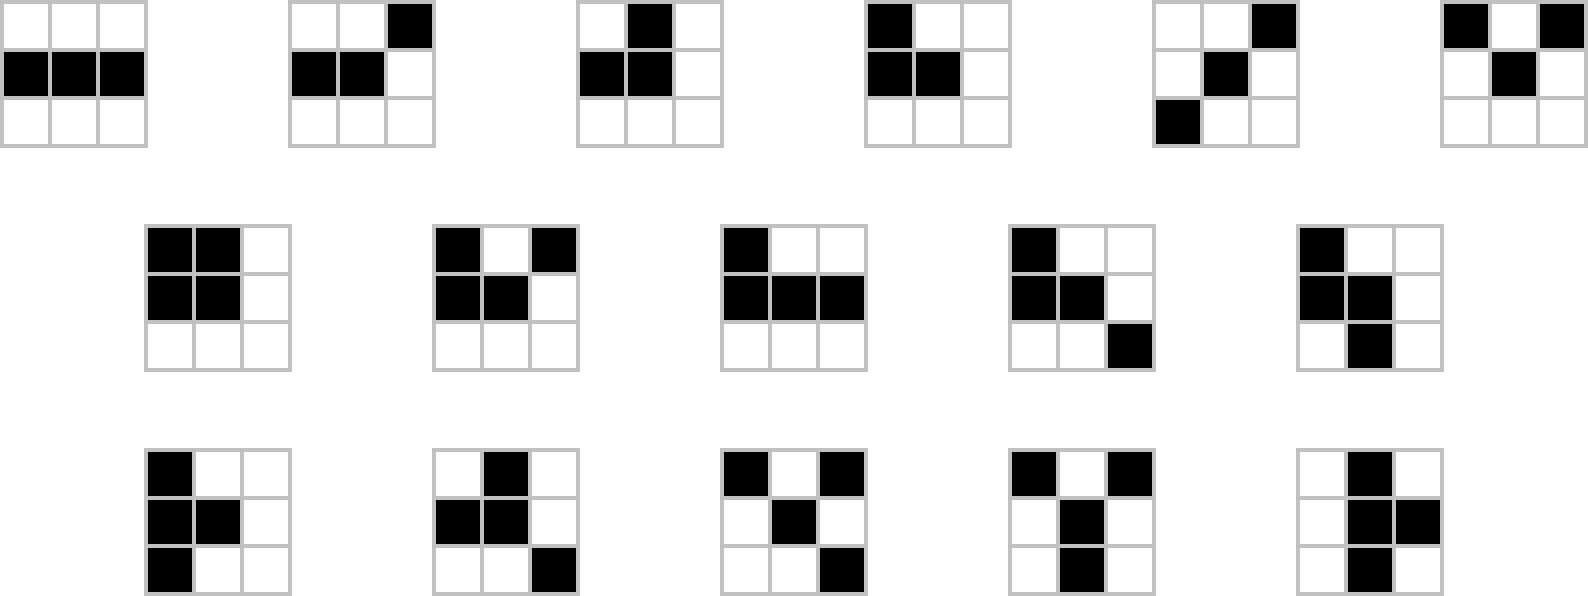
\includegraphics[width=33cm]{still_lifes/density_token_input.png}};
		
		\draw[double arrow=3pt colored by white and medgray] (1.54,12.1+2*\shftx-12) -- (1.54,13.2+2*\shftx-12);
		\draw[double arrow=3pt colored by white and medgray] (1.54,14.9+2*\shftx-12) -- (1.54,13.8+2*\shftx-12);
		\colorletternode{greenback2}{1.54}{1.5+2*\shftx}{4};
		
		\draw[double arrow=3pt colored by white and medgray] (7.54,12.1+2*\shftx-12) -- (7.54,13.2+2*\shftx-12);
		\draw[double arrow=3pt colored by white and medgray] (7.54,14.9+2*\shftx-12) -- (7.54,13.8+2*\shftx-12);
		\draw[double arrow=3pt colored by white and medgray] (8.9,13.54+2*\shftx-12) -- (7.8,13.54+2*\shftx-12);
		\colorletternode{greenback2}{7.54}{1.5+2*\shftx}{5};
		
		\draw[double arrow=3pt colored by white and medgray] (13.55,12.1+2*\shftx-12) -- (13.55,13.2+2*\shftx-12);
		\draw[double arrow=3pt colored by white and medgray] (14.91,13.54+2*\shftx-12) -- (13.81,13.54+2*\shftx-12);
		\colorletternode{greenback2}{13.55}{1.5+2*\shftx}{4};
		
		\draw[double arrow=3pt colored by white and medgray] (19.55,12.1+2*\shftx-12) -- (19.55,13.2+2*\shftx-12);
		\draw[double arrow=3pt colored by white and medgray] (19.55,14.9+2*\shftx-12) -- (19.55,13.8+2*\shftx-12);
		\draw[double arrow=3pt colored by white and medgray] (20.91,13.54+2*\shftx-12) -- (19.81,13.54+2*\shftx-12);
		\colorletternode{greenback2}{19.55}{1.5+2*\shftx}{5};
		
		\draw[double arrow=3pt colored by white and medgray] (25.52,12.1+2*\shftx-12) -- (25.52,13.2+2*\shftx-12); % d to u
		\draw[double arrow=3pt colored by white and medgray] (25.52,14.9+2*\shftx-12) -- (25.52,13.8+2*\shftx-12); % u to d
		\draw[double arrow=3pt colored by white and medgray] (26.88,13.54+2*\shftx-12) -- (25.78,13.54+2*\shftx-12); % r to l
		\draw[double arrow=3pt colored by white and medgray] (24.08,13.54+2*\shftx-12) -- (25.18,13.54+2*\shftx-12); % l to r
		\colorletternode{greenback2}{25.52}{1.5+2*\shftx}{6};
		
		\draw[double arrow=3pt colored by white and medgray] (31.52,12.1+2*\shftx-12) -- (31.52,13.2+2*\shftx-12);
		\draw[double arrow=3pt colored by white and medgray] (32.88,13.54+2*\shftx-12) -- (31.78,13.54+2*\shftx-12);
		\draw[double arrow=3pt colored by white and medgray] (30.08,13.54+2*\shftx-12) -- (31.18,13.54+2*\shftx-12);
		\colorletternode{greenback2}{31.5}{1.5+2*\shftx}{5};
		
		\draw[double arrow=3pt colored by white and medgray] (4.52,6.1+\shftx-6) -- (4.52,7.2+\shftx-6);
		\draw[double arrow=3pt colored by white and medgray] (5.88,7.54+\shftx-6) -- (4.78,7.54+\shftx-6);
		\colorletternode{greenback2}{4.52}{1.5+\shftx}{4};
		
		\draw[double arrow=3pt colored by white and medgray] (10.52,6.1+\shftx-6) -- (10.52,7.2+\shftx-6);
		\draw[double arrow=3pt colored by white and medgray] (11.88,7.54+\shftx-6) -- (10.78,7.54+\shftx-6);
		\colorletternode{greenback2}{10.52}{1.5+\shftx}{4};
		
		\draw[double arrow=3pt colored by white and medgray] (16.52,6.1+\shftx-6) -- (16.52,7.2+\shftx-6); % d to u
		\draw[double arrow=3pt colored by white and medgray] (16.52,8.9+\shftx-6) -- (16.52,7.8+\shftx-6); % u to d
		\colorletternode{greenback2}{16.52}{1.5+\shftx}{4};
		
		\draw[double arrow=3pt colored by white and medgray] (22.52,6.1+\shftx-6) -- (22.52,7.2+\shftx-6); % d to u
		\draw[double arrow=3pt colored by white and medgray] (22.52,8.9+\shftx-6) -- (22.52,7.8+\shftx-6); % u to d
		\draw[double arrow=3pt colored by white and medgray] (23.88,7.54+\shftx-6) -- (22.78,7.54+\shftx-6); % r to l
		\colorletternode{greenback2}{22.49}{1.5+\shftx}{5};
		
		\draw[double arrow=3pt colored by white and medgray] (28.52,8.9+\shftx-6) -- (28.52,7.8+\shftx-6); % u to d
		\draw[double arrow=3pt colored by white and medgray] (29.88,7.54+\shftx-6) -- (28.78,7.54+\shftx-6); % r to l
		\colorletternode{greenback2}{28.49}{1.5+\shftx}{4};
		
		\draw[double arrow=3pt colored by white and medgray] (4.52,0.1) -- (4.52,1.2); % d to u
		\draw[double arrow=3pt colored by white and medgray] (4.52,2.92) -- (4.52,1.82); % u to d
		\draw[double arrow=3pt colored by white and medgray] (5.9,1.54) -- (4.8,1.54); % r to l
		\colorletternode{greenback2}{4.52}{1.5}{5};
		
		\draw[double arrow=3pt colored by white and medgray] (10.52,0.1) -- (10.52,1.2); % d to u
		\draw[double arrow=3pt colored by white and medgray] (11.9,1.54) -- (10.8,1.54); % r to l
		\colorletternode{greenback2}{10.52}{1.5}{4};
		
		\draw[double arrow=3pt colored by white and medgray] (16.52,0.1) -- (16.52,1.2); % d to u
		\draw[double arrow=3pt colored by white and medgray] (15.1,1.54) -- (16.2,1.54); % l to r
		\colorletternode{greenback2}{16.52}{1.5}{4};
		
		\draw[double arrow=3pt colored by white and medgray] (23.9,1.54) -- (22.8,1.54); % r to l
		\draw[double arrow=3pt colored by white and medgray] (21.1,1.54) -- (22.2,1.54); % l to r
		\colorletternode{greenback2}{22.49}{1.5}{4};
		
		\draw[double arrow=3pt colored by white and medgray] (27.1,1.54) -- (28.2,1.54); % l to r
		\colorletternode{greenback2}{28.49}{1.5}{3};
		\end{tikzpicture}
		\caption{All $16$ possible orientations of $2$ or $3$ live neighbors around a live cell, up to rotation and reflection. The \bgbox{medgray!60}{dark gray} arrows indicate which of its neighboring dead cells give tokens to it. The number of tokens that end up on the central live cell is indicated in \bgbox{greenback}{green}, and is always $2$ more than the number of arrows pointing to that cell. The one problematic configuration that results in the central live cell having fewer than $4$ tokens is the one at the bottom-right, outlined in \bgbox{redback}{red}, but it can be fixed with the configuration at the bottom-left, outlined in \bgbox{yellowback2}{yellow}.}\label{fig:density_token_input}
	\end{figure}
	
	We see that in $15$ of the $16$ cases, the live cells ends up having at least $4$ tokens, as desired. However, the configuration at the bottom-right of Figure~\ref{fig:density_token_input} (outlined in red) results in the live cell only having $3$ tokens. To fix this problematic configuration, we claim that it must always be directly to the left of the configuration at the bottom-left of Figure~\ref{fig:density_token_input} (outlined in yellow). To see why this claim is true, notice that the middle-right live cell in the red configuration already has $3$ live neighbors, so the $3$ cells to its immediate right must be dead so as to avoid a birth---in other words, this cell is the central cell in the yellow configuration. In the other direction, notice that the middle-left live cell in the yellow configuration already has $3$ live neighbors, so the $3$ cells to its immediate left must be dead so as to avoid it dying---in other words, this cell is the central cell in the red configuration.
	
	We have thus shown that the red and yellow configurations always occur together. We can thus simply transfer one of the tokens from the cell with $5$ tokens to the cell with $3$ tokens, resulting in every live cell having at least $4$ tokens (see Figure~\ref{fig:density_token_input_fix}), as desired. Since we have redistributed the tokens in such a way that every live cell now has at least $4$ tokens, and no token has traveled outside of its original von Neumann neighborhood, we are done.
\end{proof}

\begin{figure}[!htb]
	\centering
	\begin{minipage}[b]{0.46\textwidth}
		\centering
		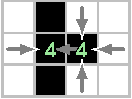
\includegraphics[scale=1.25]{still_lifes/token_redist.pdf}
		\caption{To fix the configuration from Figure~\ref{fig:density_token_input} that results in a live cell only having $3$ tokens, we transfer an extra token from a bordering live cell that has $5$.}\label{fig:density_token_input_fix}
	\end{minipage}\hfill
	\begin{minipage}[b]{0.51\textwidth}
		\centering
		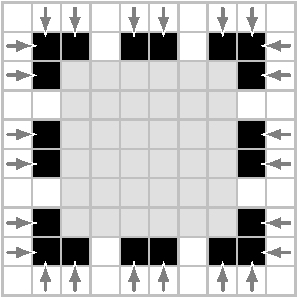
\includegraphics[scale=0.7]{still_lifes/token_dist_border.pdf}
		\caption{This border configuration is the one that causes the largest number of tokens to enter the $n \times n$ square: $4\lceil 2n/3\rceil$ (the $n = 8$ case is illustrated here, so $4\lceil 16/3 \rceil = 24$ tokens enter the square region).}\label{fig:density_border_improve}
	\end{minipage}
\end{figure}

One interesting feature of the proof of Theorem~\ref{thm:still_life_density} is that it tells us which $3 \times 3$ subpatterns of still lifes are the best at being packed densely: the patterns that result in the central cell having exactly $4$ tokens. For example, every single live cell in the infinite still lifes in Figure~\ref{fig:dense_still_lifes} ends up with exactly $4$ tokens. Similarly, it is straightforward to check that the densest still life in a $3 \times 3$ square is the ship\index{ship} (see Table~\ref{tab:still_life_n10}), and every live cell in the ship also ends up with exactly $4$ tokens. By contrast, each live cell in the tub (a less dense $3 \times 3$ still life) ends up with $5$ tokens.

While it is nice to have an answer to the asymptotic version of the still life density problem, Theorem~\ref{thm:still_life_density} does quite poorly at bounding the maximum number of cells in a given (finite) $n \times n$ square. For example, in the $n = 3$ case, that theorem says that a still life cannot have more than $10$ live cells, which is trivially true since a $3 \times 3$ square only has $9$ squares anyway. To improve the bound provided by the theorem, we note that our upper bound on the number of tokens that end up in the $n \times n$ square ($2n^2 + 8n$) can be improved without too much difficulty. In particular, far fewer than $8n$ tokens can actually enter the square from the $4n$ dead cells that neighbor it---this is because our token redistribution procedure never sends both of the tokens from one dead cell in the same direction, so in fact at most $4n$ tokens ($1$ token from each neighboring cell) can enter the square.

In fact, even this bound can be improved, because these $4n$ neighboring dead cells only send a token into the square if their neighbor inside the square is alive. However, only $2$ out of every $3$ cells on the outer edge of the square can be alive, or else they would cause a birth outside of the square and hence not be a still life. It follows that at most $4\lceil 2n/3 \rceil$ tokens can enter the square (see Figure~\ref{fig:density_border_improve}). If we repeat the calculation that was done at the start of the proof of Theorem~\ref{thm:still_life_density}, we immediately arrive at the following result, which is possibly the best upper bound on the density of a finite still life that can be ``easily'' derived:

\begin{proposition}\label{prop:still_life_density_better}
	A still life contained in an $n \times n$ bounding box has no more than $\lfloor n^2/2 \rfloor + \lceil 2n/3 \rceil$ live cells.
\end{proposition}

For large values of $n$, this new bound is not too much better than the bound provided by Theorem~\ref{thm:still_life_density}, since the $n^2/2$ term is much larger than the $2n$ term that we improved anyway. However, for small values of $n$ this bound is now good enough that it is sometimes exactly correct. In particular, when $n = 2, 3,$ or $5$, this bound equals $4$, $6$, and $16$, respectively, and it is straightforward to construct still lifes that attain these bounds---a block, a ship, and a $2 \times 2$ arrangement of $4$ blocks. For other small squares, we can find the densest still lifes simply by brute-force search: Table~\ref{tab:still_life_n10} gives a summary of the densest patterns in $n \times n$ bounding boxes for $n = 2, 3, 4, \ldots, 10$.

\begin{table}[!htb]\vspace*{0.05in}
	\begin{center}		
		\begin{tabular}{Sc Sc Sl Sc Sc Sc}
			\toprule
			$n$ & \multicolumn{2}{c}{Densest Still Life} & Prop.~\ref{prop:still_life_density_better} Bound & Maximal Live Cells & Density \\\midrule
			\specialcell{2} & \specialcell{\patternimglink{0.1969696969}{densest_block}} & \specialcell{block} & \specialcell{4} & \specialcell{4} & \specialcell{$2/2 = 1.000$} \\
			\rowcolor{gray!20} \specialcell{3} & \specialcell{\patternimglink{0.15853658536}{densest_ship}} & \specialcell{ship} & \specialcell{6} & \specialcell{6} & \specialcell{$6/9 \approx 0.6667$} \\
			\specialcell{4} & \specialcell{\patternimglink{0.13265306122}{densest_pond}} & \specialcell{pond} & \specialcell{11} & \specialcell{8} & \specialcell{$8/16 = 0.5000$} \\
			\rowcolor{gray!20} \specialcell{5} & \specialcell{\patternimglink{0.11403508771}{densest_four_blocks}} & \specialcell{four blocks} & \specialcell{16} & \specialcell{16} & \specialcell{$16/25 = 0.6400$} \\
			\specialcell{6} & \specialcell{\patternimglink{0.1}{densest_6}} & \specialcell{blocks and ship} & \specialcell{22} & \specialcell{18} & \specialcell{$18/36 = 0.5000$} \\
			\rowcolor{gray!20} \specialcell{7} & \specialcell{\patternimglink{0.08904109589}{densest_7}} & \specialcell{--} & \specialcell{29} & \specialcell{28} & \specialcell{$28/49 \approx 0.5714$} \\
			\specialcell{8} & \specialcell{\patternimglink{0.08024691358}{densest_8}} & \specialcell{nine blocks} & \specialcell{38} & \specialcell{36} & \specialcell{$36/64 = 0.5625$} \\
			\rowcolor{gray!20} \specialcell{9} & \specialcell{\patternimglink{0.07303370786}{densest_9}} & \specialcell{--} & \specialcell{46} & \specialcell{43} & \specialcell{$43/81 \approx 0.5309$} \\
			\specialcell{10} & \specialcell{\patternimglink{0.06701030927}{densest_10}} & \specialcell{--} & \specialcell{57} & \specialcell{54} & \specialcell{$54/100 = 0.5400$} \\\bottomrule
		\end{tabular}
		\caption{The densest still lifes that fit within an $n \times n$ bounding box for $2 \leq n \leq 10$, as well as the upper bound on the population of such a still life guaranteed by Proposition~\ref{prop:still_life_density_better}. The examples displayed here are only unique when $n = 2, 3, 5$, or $7$.}\label{tab:still_life_n10}
	\end{center}
\end{table}

Remarkably, we actually know a complete answer to the question of how many live cells a still life in an $n \times n$ bounding box can have. Various clever computer searches were used\footnote{These values for $n \leq 10$ were computed by Robert Bosch in 1999 \cite{Bos99}. This was extended to $n \leq 15$ by Bosch and Michael Trick in 2004 \cite{BT04}, and to $n \leq 20$ by Javier Larrosa, Enric Morancho, and David Niso in 2005 \cite{LMN05}. The remaining values were computed by Geoffrey Chu et. al., with the $n \leq 27$ values being computed in 2009 \cite{CSB09}, and a complete solution for all $n$ being presented in 2012 \cite{CS12}.} to compute the answer when $n \leq 60$, the results of which are summarized in Table~\ref{tab:still_life_n60}. For the $n \geq 61$ cases, the problem stabilizes quite a bit, and there is an explicit formula that is summarized by the following theorem. Proving this theorem is beyond the scope of this book, so the interested reader is directed to \cite{CS12} for details of how it was derived. It is worth noting that the bound we proved in Proposition~\ref{prop:still_life_density_better} is not too far from optimal: the $n^2/2$ term is right, and the linear term in our bound is $2n/3 \approx 0.6667n$, versus the following exact result which has a linear term of $17n/27 \approx 0.6296n$.

\begin{table}[!htb]\vspace*{0.05in}\setlength\arrayrulewidth{0.75pt}
	\begin{center}		
		\begin{tabular}{c | c c c c c c}
			\toprule
			$n$ & $M(n)$ & $M(n+10)$ & $M(n+20)$ & $M(n+30)$ & $M(n+40)$ & $M(n+50)$ \\ \midrule
			$1$ & $0$ & $64$ & $232$ & $497$ & $864$ & $1,331$ \\
			\rowcolor{gray!20} $2$ & $4$ & $76$ & $253$ & $531$ & $907$ & $1,382$ \\
			$3$ & $6$ & $90$ & $276$ & $563$ & $949$ & $1,436$ \\
			\rowcolor{gray!20} $4$ & $8$ & $104$ & $302$ & $598$ & $993$ & $1,490$ \\
			$5$ & $16$ & $119$ & $326$ & $633$ & $1,039$ & $1,545$ \\
			\rowcolor{gray!20} $6$ & $18$ & $136$ & $353$ & $668$ & $1,085$ & $1,602$ \\
			$7$ & $28$ & $152$ & $379$ & $706$ & $1,132$ & $1,658$ \\
			\rowcolor{gray!20} $8$ & $36$ & $171$ & $407$ & $744$ & $1,181$ & $1,717$ \\
			$9$ & $43$ & $190$ & $437$ & $782$ & $1,229$ & $1,776$ \\
			\rowcolor{gray!20} $10$ & $54$ & $210$ & $467$ & $824$ & $1,280$ & $1,835$ \\
			\bottomrule
		\end{tabular}
		\caption{A summary of the maximum number of live cells $M(n)$ in a still life with an $n \times n$ bounding box for $1 \leq n \leq 60$.}\label{tab:still_life_n60}
	\end{center}
\end{table}

\begin{theorem}\label{thm:still_life_density_finite}
	For all $n \geq 61$, the maximum number of live cells $M(n)$ in a still life with an $n \times n$ bounding box is given by the formula
	$$
	M(n) = \begin{cases}
	\lfloor n^2/2 + 17n/27 - 2 \rfloor, & \text{ if } n \equiv 0, 1, 3, 8, 9, 11, 16, 17, 19, 25, 27, \\
	& \quad \quad \ \ \ \, 31, 33, 39, 41, 47, \text{or } 49 \ (\text{mod } 54) , \text{ and} \\
	\lfloor n^2/2 + 17n/27 - 1 \rfloor, & \text{ otherwise}.
	\end{cases}
	$$
\end{theorem}

The related problem of finding the maximum density of an oscillator remains open, even in the (presumably) simpler case of infinite oscillators. Although it is possible for oscillators to have individual phases with density higher than $1/2$ (see Figure~\ref{fig:dense_oscillator} for an example), it seems that their average density over all of their phases is never greater than $1/2$, just like still lifes. Unfortunately, none of the three known proof techniques for the still life case (i.e., the method introduced by Elkies in \cite{Elk98}, the method we used to prove Theorem~\ref{thm:still_life_density}, and the computer-assisted method that was used to prove Theorem~\ref{thm:still_life_density_finite} in \cite{CS12}) seem to carry over in a straightforward way to oscillators.

\begin{figure}[!htb]
	\centering
	\embedlink{dense_oscillator}{\vcenteredhbox{\patternimg{0.1}{dense_oscillator_0}} \vcenteredhbox{\genarrow{1}} \vcenteredhbox{\patternimg{0.1}{dense_oscillator_1}} \vcenteredhbox{\genarrow{1}} \vcenteredhbox{\patternimg{0.1}{dense_oscillator_2}} \vcenteredhbox{\genarrow{1}} \vcenteredhbox{\patternimg{0.1}{dense_oscillator_3}} \vcenteredhbox{\genarrow{1}} \vcenteredhbox{\patternimg{0.1}{dense_oscillator_4}} \vcenteredhbox{\genarrow{1}} \vcenteredhbox{\patternimg{0.1}{dense_oscillator_5}}}
	\caption{A period~$6$ infinite oscillator that has density $3/4$ in two of its phases. However, its average density over all of its phases is $(3/4 + 1/4 + 1/4 + 3/4 + 1/4 + 1/4)/6 = 5/12 \leq 1/2$.}\label{fig:dense_oscillator}
\end{figure}

We could also ask for the densest possible individual phase of an oscillator. It is suspected that the highest possible density is $3/4$, which is attained by some of the phases of the oscillator in Figure~\ref{fig:dense_oscillator}, but no proof of this conjecture has been found either.


%%%%%%%%%%%%%%%%%%%%%%%%%%%%%%%%%%%%%%%%%%%%%%%%%%%%%%%%%%%%%%%%%%%%%%%%%
%%   SECTION: NOTES AND HISTORICAL REMARKS
%%
%%   http://codercontest.com/mniemiec/lifemeth.htm
%%   http://wwwhomes.uni-bielefeld.de/achim/still_life.html
%%%%%%%%%%%%%%%%%%%%%%%%%%%%%%%%%%%%%%%%%%%%%%%%%%%%%%%%%%%%%%%%%%%%%%%%%
\section*{Notes and Historical Remarks}
\label{sec:still_lifes_notes}
\addcontentsline{toc}{section}{\nameref{sec:still_lifes_notes}}
%%%%%%%%%%%%%%%%%%%%%%%%%%%%%%%%%%%%%%%%%%%%%%%%%%%%%%%%%%%%%%%%%%%%%%%%%

Right from the early days of Life, there was considerable interest in cataloging all small still lifes. This process was initiated by John Conway himself, who enumerated the still lifes with $7$ or fewer live cells. Robert Wainwright, with the help of the Life community, then constructed all of them with $10$ or fewer live cells by hand (see Figure~\ref{fig:sl_table_inc}). This effort was soon extended to $12$ cells by Douglas Petrie and Everett Boyer (see Figure~\ref{fig:12_cell_sl_table}). David Buckingham independently went as high as $13$ cells, which we recall there are $240$ of, so cataloging them all by hand (and being sure that none were missed!) was no small feat. Peter Raynham then wrote a search program in the mid-1970s that verified the $13$-cell still life counts and was also used by Buckingham to find all $14$-cell strict still lifes.\index{Lifeline}

\begin{figure}[!htb]
	\centering
	\begin{minipage}[b]{0.48\textwidth}
		\centering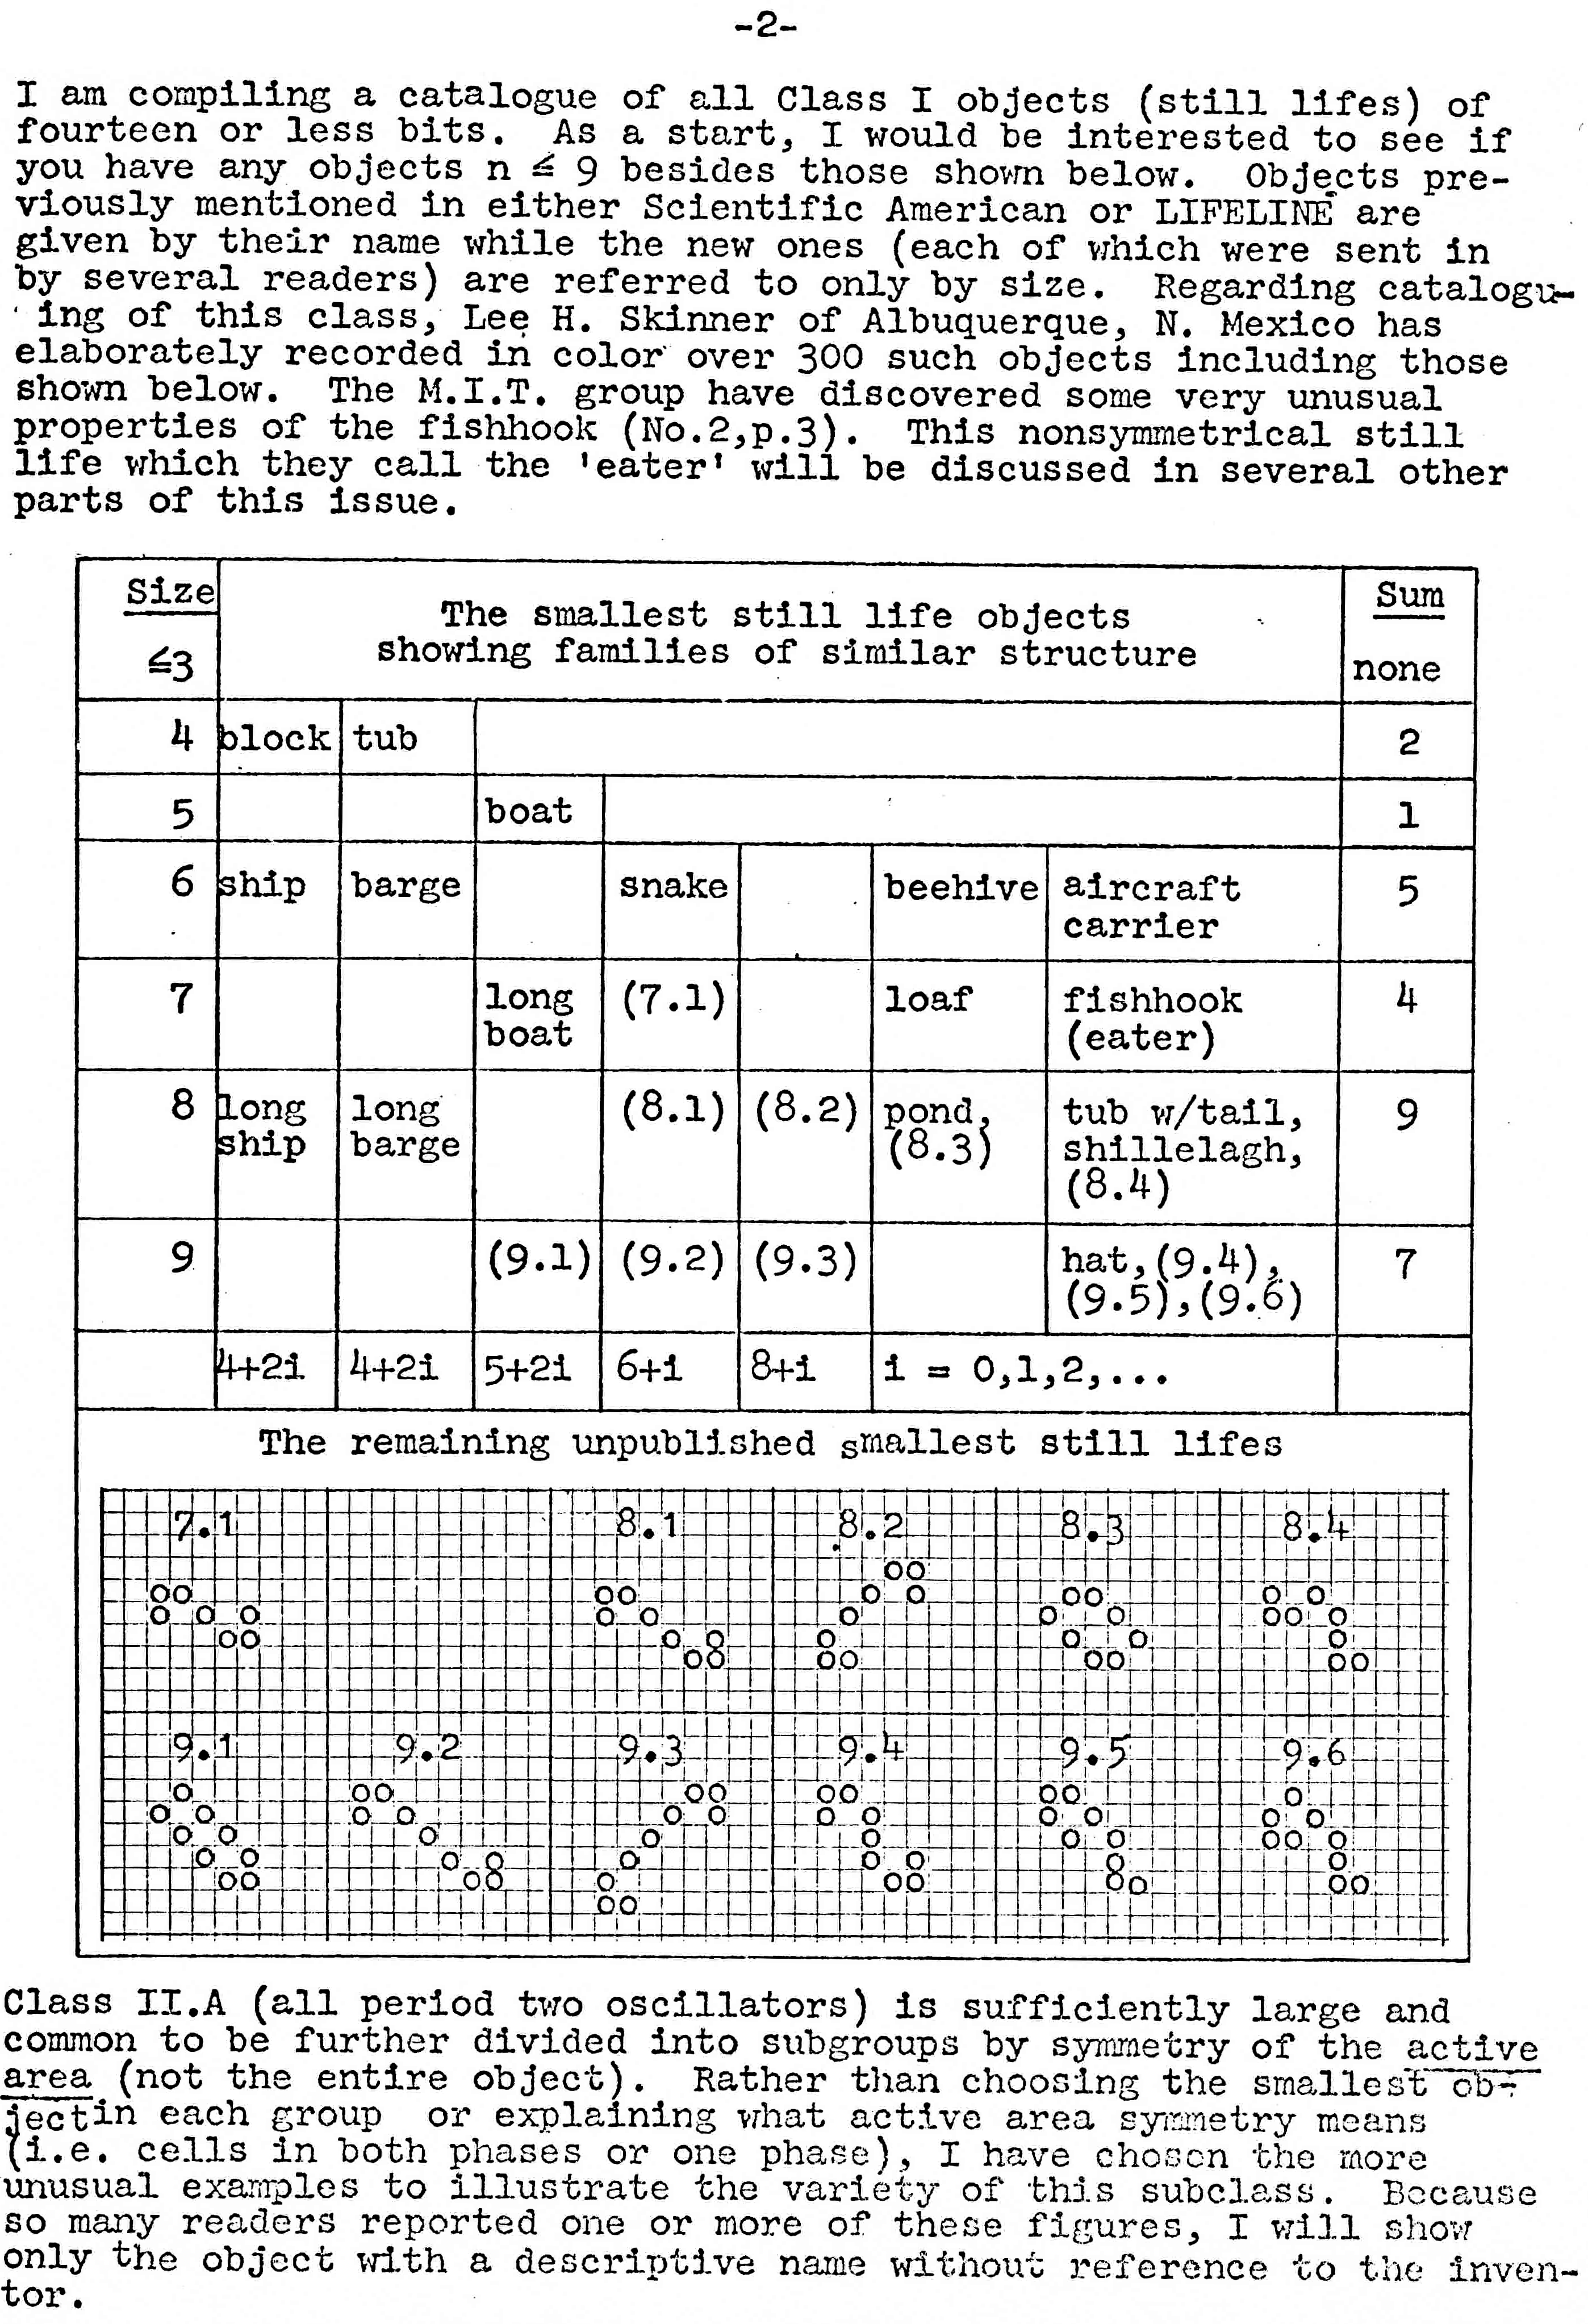
\includegraphics[width=0.75\textwidth]{still_lifes/sl_table_inc.png}
		\caption{A summary of all strict still lifes with $8$ or fewer cells, and an incomplete summary of just $6$ (out of $10$) of the $9$-cell still lifes. Originally published in \emph{Lifeline} vol.~3 in September~1971.}\label{fig:sl_table_inc}
	\end{minipage}\hfill
	\begin{minipage}[b]{0.48\textwidth}
		\centering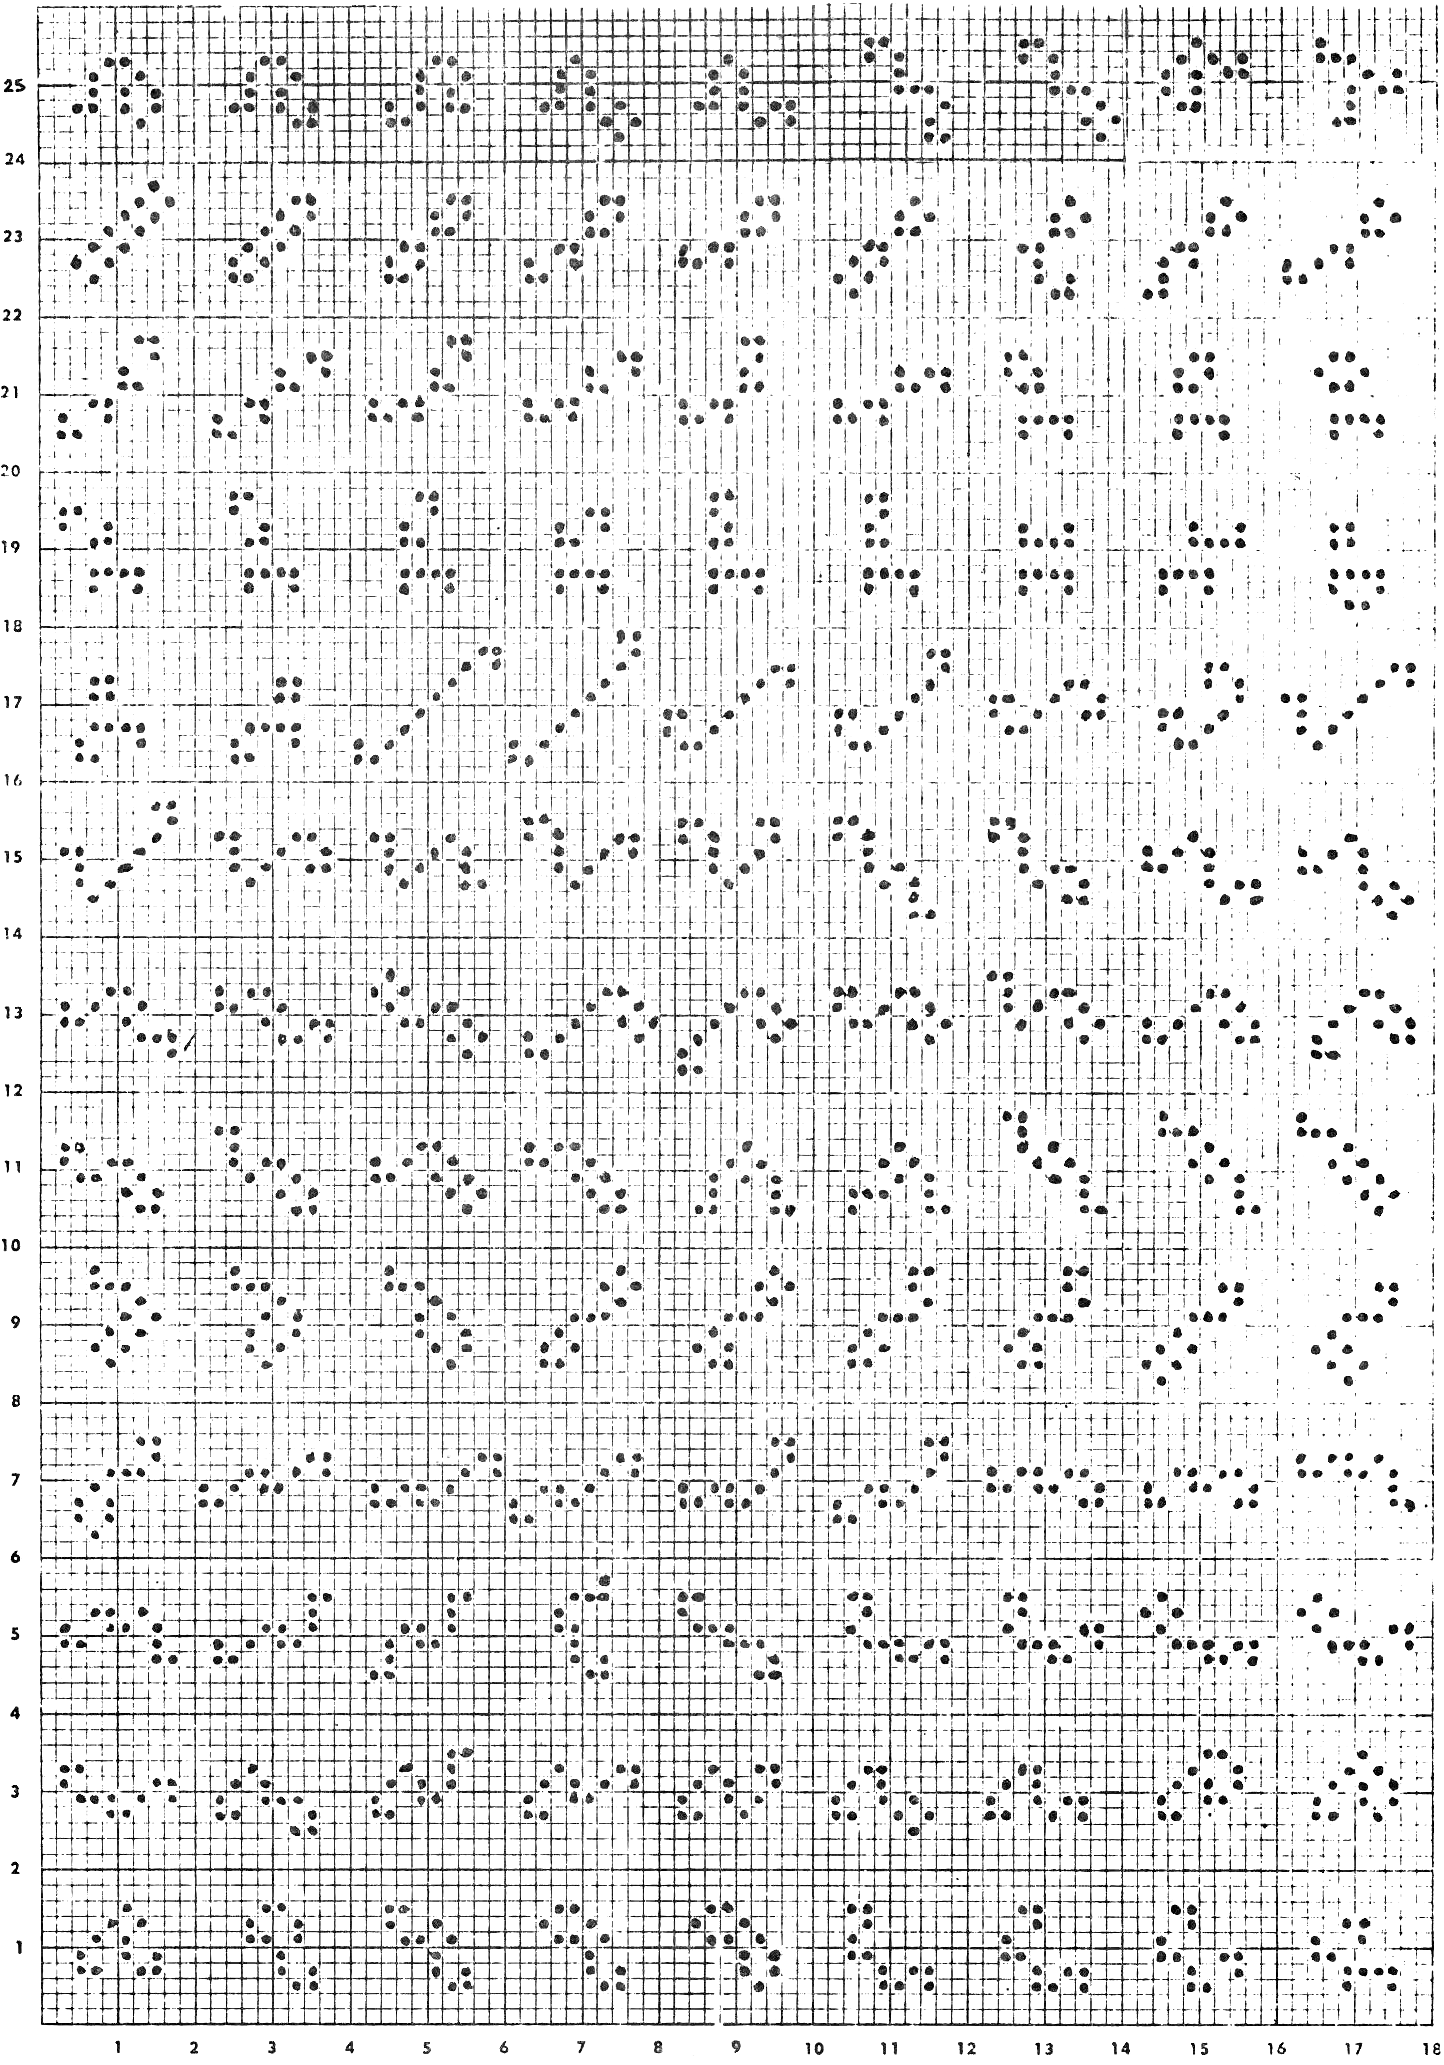
\includegraphics[width=0.75\textwidth]{still_lifes/12_cell_sl_table.png}
		\caption{A summary of all $121$ distinct $12$-cell strict still lifes, compiled by hand by Douglas Petrie and Everett Boyer in 1973. Originally published in \emph{Lifeline} vol.~10 in June~1973.}\label{fig:12_cell_sl_table}
	\end{minipage}
\end{figure}

Much of the early difficulty with counting still lifes with more than $14$ cells came not just from the fact that the search space was large, but also from the fact that even knowing \emph{how} to search for larger still lifes becomes increasingly complicated. To give an idea of why this is the case, suppose we tried to construct strict still lifes by starting at their top-left corner, placing live cells one at a time, checking whether the resulting pattern is stable after each new cell is added. It might seem reasonable to guess that there is no reason to add additional nearby objects once we find a strict still life, since the resulting pattern would then be a pseudo still life. However, this is not actually the case: there are strict still lifes that will never be found if we stop the search when we first find stability, the smallest of which has $16$ cells and is displayed in Figure~\ref{fig:two_tables_on_block}.

\begin{figure}[!htb]
	\centering
	\begin{minipage}{.42\textwidth}
		\centering
		\patternimglink{0.11}{two_tables_on_block}
		\caption{A strict still life that would never be found via a greedy still life search, since a block on table would be found before adding the second table.}\label{fig:two_tables_on_block}
	\end{minipage} \hfill %
	\begin{minipage}{.54\textwidth}
		\centering
		\patternimglink{0.1}{sl_hard_to_find}
		\caption{Two more strict still lifes that won't be found by a greedy still life search, and had to be added by hand when cataloging all still lifes with $22$--$24$ cells.}\label{fig:sl_hard_to_find}
	\end{minipage}
\end{figure}

This problem is not \emph{too} difficult to get around, as there are still only a few different ways that connected components can be near each other, and they can each be coded into the search algorithm individually. For example, objects like the one in Figure~\ref{fig:two_tables_on_block} can be found by allowing the search to add a new domino near an already-stable domino part of the still life. However, each of these tweaks to the algorithm makes it more complicated and thus increases its running time.

Using these ideas, Mark Niemiec conducted a very successful still life search, cataloging all of them with $24$ or fewer live cells by 1999. However, even his searches were not perfect; they missed some still lifes that use a single cell to stabilize a long line of orthogonally-connected cells, like the one in Figure~\ref{fig:sl_hard_to_find}. These still lifes had to be added back into the count by hand, and they were the main reason why he did not extend his search to $25$-cell still lifes---the number of exceptional still lifes that would need to be added back in by hand is too large, and could potentially lead to errors.\footnote{In fact, even after the manual corrections to his $24$-cell still life counts, it was discovered in 2017 that six $24$-cell strict still lifes and one $24$-cell pseudo still life had been missed.}

Finally, Simon Ekström wrote a program to search for still lifes in January 2017 that led to the most successful still life search to date.\footnote{His program is available online at \httpsurl{github.com/simeksgol/GoL_still_life_searcher}} This program has now been used to catalog all still lifes (both strict and pseudo) with $30$ or fewer cells, count all still lifes with $34$ or fewer cells, and also show that the pseudo still lifes from Figure~\ref{fig:pseudo_still_life_decompose} that can be partitioned into $3$ or $4$ still lifes, but not $2$, are the smallest ones possible.


%%%%%%%%%%%%%%%%%%%%%%%%%%%%%%%%%
\section*{Exercises \hfill \normalfont\textsf{\small solutions to starred exercises on \hyperlink{solutions_still_lifes}{page \pageref{solutions_still_lifes}}}}
\label{sec:still_lifes_exercises}
\addcontentsline{toc}{section}{Exercises}
\vspace*{-0.4cm}\hrulefill\vspace*{-0.3cm}\footnotesize\begin{multicols}{2}\vspace*{-0.4cm}\raggedcolumns\interlinepenalty=10000
	\setlength{\parskip}{0pt}
	%%%%%%%%%%%%%%%%%%%%%%%%%%%%%%%%%
	
	\begin{problemstar}\label{exer:classify_still_lifes}
		Classify each of the following still lifes as either a strict still life, a pseudo still life, or neither.\setlength{\columnsep}{0pt}\vspace*{-0.25cm}
		
		\begin{multicols}{2}
			\begin{enumerate}
				\item[\bf\color{ocre}(a)] \raisebox{-\height+0.5em}{\patternimglink{0.1}{exercise_strict_pseudo_1}}\\[0.2em]
				
				\item[\bf\color{ocre}(c)] \raisebox{-\height+0.5em}{\patternimglink{0.1}{exercise_strict_pseudo_2}}\\[0.9em]
				
				\item[\bf\color{ocre}(e)] \raisebox{-\height+0.5em}{\patternimglink{0.1}{exercise_strict_pseudo_3}}
				
				\item[\bf\color{ocre}(b)] \raisebox{-\height+0.5em}{\patternimglink{0.085}{exercise_strict_pseudo_4}}
				
				\item[\bf\color{ocre}(d)] \raisebox{-\height+0.5em}{\patternimglink{0.085}{exercise_strict_pseudo_5}}
				
				\item[\bf\color{ocre}(f)] \raisebox{-\height+0.5em}{\patternimglink{0.1}{exercise_strict_pseudo_6}}
			\end{enumerate}
		\end{multicols}
	\end{problemstar}
	
	
	\mfilbreak
	
	
	\begin{problem}\label{exer:quasi_still_life}
		A \emph{quasi still life}\index{quasi still life} is a still life that can be partitioned into two or more disjoint still lifes with overlapping Moore neighborhoods (just like pseudo still lifes), but with all cells that stay dead from underpopulation in the constituent still lifes remaining underpopulated in the overall pattern. For example, the cell highlighted in \bgbox{yellowback2}{yellow} in Figure~\ref{fig:pseudo_not_pseudo} makes that configuration of two blocks a quasi still life.\smallskip
		
		\begin{enumerate}[label=\bf\color{ocre}(\alph*)]
			\item Which of the still lifes from Exercise~\ref{exer:classify_still_lifes} is a quasi still life?
			
			\item Show how to partition the following configuration of $4$ blocks into...
			
			\begin{center}
				\patternlink{densest_four_blocks}{\patternimg{0.1}{densest_four_blocks}}
			\end{center}
			
			\begin{enumerate}[label=\bf\color{ocre}(\roman*)]
				\item two pseudo still lifes,
				
				\item two quasi still lifes, and
				
				\item a quasi still life and two strict still lifes.
			\end{enumerate}
		\end{enumerate}
	\end{problem}
	
	
	\mfilbreak
	
	
	\begin{problemstar}\label{exer:pseudo_few_colors}
		Partition each of the following pseudo still lifes into the smallest number (either $2$, $3$, or $4$) of still lifes possible.\setlength{\columnsep}{0pt}\vspace*{-0.25cm}
		
		\begin{multicols}{2}
			\begin{enumerate}[label=(\alph*),series=exer_pseudo]
				\item[\bf\color{ocre}(a)] \raisebox{-\height+0.5em}{\patternimglink{0.1}{exercise_pseudo_1}}
				
				\item[\bf\color{ocre}(c)] \raisebox{-\height+0.5em}{\patternimglink{0.1}{exercise_pseudo_2}}\\[1.0em]
				
				\item[\bf\color{ocre}(e)] \raisebox{-\height+0.5em}{\patternimglink{0.1}{exercise_pseudo_3}}
				
				\item[\bf\color{ocre}(b)] \raisebox{-\height+0.5em}{\patternimglink{0.09}{exercise_pseudo_4}}
				
				\item[\bf\color{ocre}(d)] \raisebox{-\height+0.5em}{\patternimglink{0.085}{exercise_pseudo_5}}
				
				\item[\bf\color{ocre}(f)] \raisebox{-\height+0.5em}{\patternimglink{0.09}{exercise_pseudo_6}}
			\end{enumerate}
		\end{multicols}
	\end{problemstar}
	
	
	\mfilbreak
	
	
	\begin{problemstar}\label{exer:still_life_add_dead}
		For each of the following patterns, find a way of changing some nearby dead cells into alive cells so that the resulting pattern is a still life (similarly to how we turned in the path in Figure~\ref{fig:still_life_path} into a still life).\vspace*{-0.25cm}
		
		\begin{multicols}{2}
			\begin{enumerate}
				\item[\bf\color{ocre}(a)] \raisebox{-\height+0.5em}{\patternimglink{0.1}{exercise_path_1}}
				
				\item[\bf\color{ocre}(c)] \raisebox{-\height+0.5em}{\patternimglink{0.1}{exercise_path_2}}
				
				\item[\bf\color{ocre}(b)] \raisebox{-\height+0.5em}{\patternimglink{0.1}{exercise_path_3}}
			\end{enumerate}
		\end{multicols}
	\end{problemstar}
	
	
	\mfilbreak
	
	
	\begin{problem}\label{exer:small_strict_still_lifes}
		Find all strict still lifes, distinct up to rotation and reflection, with:\smallskip
		
		\begin{enumerate}[label=\bf\color{ocre}(\alph*)]
			\item $8$ live cells, and
			
			\item $9$ live cells.
		\end{enumerate}
	\end{problem}
	
	
	\mfilbreak
	
	
	\begin{problem}\label{exer:small_pseudo_still_lifes}
		Find all pseudo still lifes, distinct up to rotation and reflection, with:\smallskip
		
		\begin{enumerate}[label=\bf\color{ocre}(\alph*)]
			\item $10$ live cells, and
			
			\item $11$ live cells.
		\end{enumerate}
	\end{problem}
	
	
	\mfilbreak
	
	
	\begin{problemstar}\label{exer:still_life_add_coil}
		For each of the following patterns, find a way of adding induction coils so as to create a still life.\vspace*{-0.25cm}
		
		\begin{multicols}{2}\setlength{\columnsep}{1pt}
			\begin{enumerate}[label=(\alph*),series=exer_induction_coil]
				\item[\bf\color{ocre}(a)] \raisebox{-\height+0.5em}{\patternimglink{0.1}{exercise_induction_coil_1}}
				
				\item[\bf\color{ocre}(c)] \raisebox{-\height+0.5em}{\patternimglink{0.1}{exercise_induction_coil_2}}
				
				\item[\bf\color{ocre}(b)] \raisebox{-\height+0.5em}{\patternimglink{0.1}{exercise_induction_coil_3}}
			\end{enumerate}
		\end{multicols}
	\end{problemstar}
	
	
	\mfilbreak
	
	
	\begin{problem}\label{exer:gosper_oscillator}
		Use the Gosper glider gun and an eater of your choice to create a period~30 oscillator.
	\end{problem}
	
	
	\mfilbreak
	
	
	\begin{problemstar}\label{exer:eater_weld}
		For each of the following configurations, weld or modify eater~1s and/or eater~2s so as to create a single eater that can destroy all of the displayed gliders, yet lives entirely within the region specified by the light gray cells.\vspace*{-0.25cm}
		
		\begin{enumerate}
			\begin{multicols}{2}		
				\item[\bf\color{ocre}(a)] \raisebox{-\height+0.5em}{\patternimglink{0.1}{exercise_weld_1}}\vspace*{0.1cm}
				
				\item[\bf\color{ocre}(c)] \raisebox{-\height+0.5em}{\patternimglink{0.1}{exercise_weld_5}}
				
				\item[\bf\color{ocre}(b)] \raisebox{-\height+0.5em}{\patternimglink{0.1}{exercise_weld_2}}
				
				\item[\bf\color{ocre}(d)] \raisebox{-\height+0.5em}{\patternimglink{0.1}{exercise_weld_3}}
			\end{multicols}
		\end{enumerate}
		\begin{enumerate}[label=\bf\color{ocre}(\alph*)]
			\vspace*{-0.32cm}
			\item[\bf\color{ocre}(e)] \raisebox{-\height+0.5em}{\patternimglink{0.1}{exercise_weld_4}}
			
			\item[\bf\color{ocre}(f)] \raisebox{-\height+0.5em}{\patternimglink{0.1}{exercise_weld_6}}\\
		\end{enumerate}
	\end{problemstar}
	
	
	\mfilbreak
	
	
	\begin{problem}\label{exer:eater_2_lwss_mwss}
		Show how a single eater~2\index{eater 2} can be used to eat...\smallskip
		
		\begin{enumerate}[label=\bf\color{ocre}(\alph*)]
			\item a lightweight spaceship, and
			
			\item a middleweight spaceship.
		\end{enumerate}
	\end{problem}
	
	
	\mfilbreak
	
	
	\begin{problem}\label{exer:eater_3}
		Recall \emph{eater~3}\index{eater!eater 3} from Figure~\ref{fig:eater_3}.\smallskip
		
		\begin{enumerate}[label=\bf\color{ocre}(\alph*)]
			\item Find a way to use eater~3 to eat a glider.
			
			\item Find at least two still lifes that eater~3 can also eat when they are placed near its loaf.
			
			\item Use two copies of the loaf-flipping reaction in eater~3 to create a period~$8$ oscillator.
		\end{enumerate}
		% SOLUTION:
		% x = 100, y = 43, rule = B3/S23
		% 46bobo5bo3bo$45bo3bo4bo3bo4bo$46bo7bo3bo7bo3bo$48b2ob2obo3bob2ob2obo3b
		% o4bo$54bo3bo7bo3bo7bo3bo5bobo$47bo3bo9bo4bo3bob2ob2obo3bo4bo3bo$45bobo
		% 18bo3bo7bo3bo7bo$44bo28bo4bo3bob2ob2o$47bo30bo3bo$44bobo38bo3bo$40bo3b
		% o44bobo$bobo5bo3bo19bo3bo$o3bo4bo3bo4bo9bo4bo3bob2ob2o47bo$bo7bo3bo7bo
		% 3bo7bo3bo7bo45b2o$3b2ob2obo3bob2ob2obo3bob2ob2obo3bo4bo3bo45bo$9bo3bo
		% 7bo3bo7bo3bo5bobo45bo2bo$2bo3bo9bo4bo3bo4bo63bo4bo$obo18bo3bo63b3ob2ob
		% 4o$89b4ob2ob3o$2bo86bo4bo$2b2o90bo2bo$3bo92bo$2bo2bo90b2o$5bo4bo86bo$
		% 3ob2ob4o$4ob2ob3o63bo3bo18bobo$o4bo63bo4bo3bo4bo9bo3bo$5bo2bo45bobo5bo
		% 3bo7bo3bo7bo3bo$7bo45bo3bo4bo3bob2ob2obo3bob2ob2obo3bob2ob2o$7b2o45bo
		% 7bo3bo7bo3bo7bo3bo7bo$8bo47b2ob2obo3bo4bo9bo4bo3bo4bo3bo$62bo3bo19bo3b
		% o5bobo$8bobo44bo3bo$10bo3bo38bobo$17bo3bo30bo$11b2ob2obo3bo4bo28bo$9bo
		% 7bo3bo7bo3bo18bobo$8bo3bo4bo3bob2ob2obo3bo4bo9bo3bo$9bobo5bo3bo7bo3bo
		% 7bo3bo$24bo4bo3bob2ob2obo3bob2ob2o$29bo3bo7bo3bo7bo$36bo4bo3bo4bo3bo$
		% 41bo3bo5bobo!
	\end{problem}
	
	
	\mfilbreak
	
	
	\begin{problem}\label{exer:still_life_impossible}
		Prove that it is not possible to stabilize the path of live cells displayed below into a still life, no matter what dead cells you change to alive.
		
		\begin{center}
			\patternimglink{0.1}{exercise_still_life_impossible}
		\end{center}
	\end{problem}
	
	
	\mfilbreak
	
	
	\begin{problemstar}\label{exer:fast_glider_eater}
		Show how each of the following still lifes can be used to eat a glider in only $4$ generations, tying them with eater~1 as the fastest-known glider eaters.\vspace*{-0.25cm}
		
		\begin{multicols}{2}
			\begin{enumerate}
				\item[\bf\color{ocre}(a)] \raisebox{-\height+0.5em}{\patternimglink{0.1}{fast_glider_eater}}
				
				\item[\bf\color{ocre}(b)] \raisebox{-\height+0.5em}{\patternimglink{0.1}{fast_glider_eater_b}}
			\end{enumerate}
		\end{multicols}
	\end{problemstar}
	
	
	\mfilbreak
	
	
	\begin{problem}\label{exer:loaf_eater}
		Use a single loaf to eat both of the gliders displayed in Exercise~\ref{exer:eater_weld}(a), (b), and (d).
	\end{problem}
	% x = 73, y = 15, rule = B3/S23
	% 2bo19bo$obo17bobo19bo19bo$b2o18b2o17bobo17bobo$25b2o14b2o18b2o$24bo2bo
	% 16b2o$2o22bobo16bo2bo18b2o$2o23bo17bobo18bo2bo$44bo19bobo$30b2o33bo$
	% 30bobo$30bo19b2o$50bobo17b2o$2b3o45bo19bobo$2bo67bo$3bo!
	
	
	\mfilbreak
	
	
	\begin{problemstar}\label{exer:incomplete_glider_eater}
		Complete the incomplete glider eater displayed below in such a way that it lives entirely within the region specified by the light gray cells.
		
		\begin{center}
			\patternimg{0.1}{incomplete_glider_eater}
		\end{center}
	\end{problemstar}
	
	
	\mfilbreak
	
	
	\begin{problemstar}\label{exer:still_lifes_6_neigh}
		Prove that in a still life, a dead cell can have no more than six live neighbors. Provide an example of a still life that attains this bound.
	\end{problemstar}
	
	
	\mfilbreak
	
	
	\begin{problem}\label{exer:densest_still_lifes}
		Find maximum-density still lifes in $n \times n$ bounding boxes for $n = 4, 6,$ and $8$ that are different from those displayed in Table~\ref{tab:still_life_n10}.
	\end{problem}
	
	
	\mfilbreak
	
	
	\begin{problem}\label{exer:still_life_tokens}
		In the proof of Theorem~\ref{thm:still_life_density}, we described a procedure for distributing tokens on the Life grid in such a way that every live cell in a still life ends up with at least $4$ tokens. Use this procedure to determine how many tokens end up on each live cell of the following still lifes:\smallskip
		
		\begin{enumerate}[label=\bf\color{ocre}(\alph*)]
			\item block,
			
			\item beehive,
			
			\item pond, and
			
			\item eater~1.
		\end{enumerate}
	\end{problem}
	
	
	\mfilbreak
	
	
	\begin{problemstar}\label{exer:sl_density_611}
		In the proof of Theorem~\ref{thm:still_life_density}, we described a procedure for distributing tokens on the Life grid that allowed us to prove that the asymptotic density of still lifes is no greater than $1/2$. If we instead use the much simpler token distribution scheme of ``every dead cell gives each live neighbor (in the Moore neighborhood sense) one token'', then we get a weaker upper bound, which you will now derive.\smallskip
		
		\begin{enumerate}[label=\bf\color{ocre}(\alph*)]
			\item Using this new token distribution scheme, how many tokens should each cell start with to ensure that no cell ends up with a negative number of tokens? [Hint: Use Exercise~\ref{exer:still_lifes_6_neigh}.]
			
			\item Find a lower bound on the number of tokens that each live cell receives.
			
			\item Mimic the calculation at the start of the proof of Theorem~\ref{thm:still_life_density} to conclude that the asymptotic density of a still life is no greater than $6/11$.
		\end{enumerate}
	\end{problemstar}
	
	
	\mfilbreak
	
	
	\begin{problem}\label{exer:still_life_density_rectangle}
		In this question, we will consider the problem of finding the maximum density still life in a rectangular $m \times n$ bounding box.\smallskip
		
		\begin{enumerate}[label=\bf\color{ocre}(\alph*)]
			\item Prove that a still life with an $m \times n$ bounding box cannot have more than $\lfloor mn/2 \rfloor + m + n$ live cells. [Hint: Use the token distribution scheme from the proof of Theorem~\ref{thm:still_life_density}.]
			
			\item Prove that a still life with an $m \times n$ bounding box cannot have more than $$\Big\lfloor mn/2 + \frac{1}{2}\lceil 2m/3 \rceil + \frac{1}{2}\lceil 2n/3 \rceil \Big\rfloor$$ live cells. [Hint: Use the argument that was used to prove Proposition~\ref{prop:still_life_density_better}.]
			
			\item Use the formula from part~(b) to show that a still life with an $2 \times n$ bounding box cannot have more than
			$$
			n + \big\lceil(n+2)/3\big\rceil
			$$
			live cells. Show that this bound is tight whenever $n \geq 2$ and $n \not\equiv 0 \ (\text{mod } 3)$. What do you expect the maximum number of live cells is when $n \equiv 0 \ (\text{mod } 3)$? Prove it.
			% to prove tightness when n \equiv 1 mod 3, use blocks next to each other. When n \equiv 2 mod 3, use snake and snake-like still lifes. when n = 0 mod 3, we expect it equal to n + ceil((n+2)/3) - 1 (i.e., one less than this formula)
			
			\item Write a computer program that calculates the maximum number of live cells in a still life with a $3 \times n$ bounding box for $n = 2, 3, \ldots, 10$. Compare your results with the bound from part~(b).
			% SOLUTION: 4, 6, ...? 
		\end{enumerate}
	\end{problem}
	
	
	\mfilbreak
	
	
	\begin{problem}\label{exer:dense_oscillator}
		Construct an (infinitely large) oscillator of period at least $2$ with average density over all of its phases equal to exactly $1/2$.
	\end{problem}
	
	%% EXERCISE END COMMANDS
\end{multicols}
\normalsize\vspace*{0.01cm}
%% DONE EXERCISE END COMMANDS